\documentclass[oneside,openany,a4paper,12pt]{article}

% بسته‌های ریاضی و عمومی مورد نیاز
\usepackage{amsthm,amssymb,amsmath}
\usepackage[top=30mm, bottom=25mm, left=25mm, right=30mm]{geometry}
\usepackage{graphicx}
\usepackage{framed}
\usepackage{fancyhdr}
\usepackage{setspace}
\usepackage{multirow}
\usepackage{float}
\usepackage{subfigure}
\usepackage{booktabs}

% بسته‌ و دستوراتی برای ایجاد لینک‌های رنگی
\usepackage[pagebackref=false,colorlinks,linkcolor=blue,citecolor=blue]{hyperref}

% فراخوانی بسته زی‌پرشین و تعریف قلم‌های فارسی و انگلیسی
\usepackage{xepersian}
\settextfont[Path=font/,Extension=.ttf,Scale=1.1,
    BoldFont=XB NiloofarBd,
    ItalicFont=XB NiloofarIt,
    BoldItalicFont=XB NiloofarBdIt
]{XB Niloofar}
\setlatintextfont[Scale=0.9]{Times New Roman}
\setdigitfont[Path=font/,Extension=.ttf,Scale=1.1,
    BoldFont=XB NiloofarBd,
    ItalicFont=XB NiloofarIt,
    BoldItalicFont=XB NiloofarBdIt
]{XB Niloofar}

\makeatletter
\providecommand{\AutoPersianDigits}{}
\makeatother

\begin{document}
\AutoPersianDigits
\setstretch{1.4}

\begin{center}
    \vspace*{1cm}
    \Huge\textbf{گزارش تفصیلی شبیه‌ساز مأموریت پهپاد \lr{(DARTSim)} و یکپارچه‌سازی روش \lr{RS-DRL} با حلقه \lr{MAPE-K}}
\end{center}

\newpage
\tableofcontents
\newpage

\section{مقدمه و معرفی بستر شبیه‌سازی DARTSim}
شبیه‌ساز مأموریت تاکتیکی پهپادها \lr{(DARTSim)} \cite{MorenoDART2019} یک بستر شبیه‌سازی جامع برای ارزیابی تصمیم‌گیری انطباقی در تیم‌های پهپادی است. در این سیستم، تیمی از پهپادها مأموریت پیمایش و شناسایی را در یک حریم هوایی متخاصم اجرا می‌کند. هدف، حفظ بقای تیم و بیشینه‌سازی اهداف مأموریت از طریق تصمیمات تاکتیکی است.

DARTSim بر اساس مسئله‌ی تیم پهپادهای خودگردان \lr{(UAV Team)} ساخته شده است. مورنو و همکاران \cite{moreno2015proactive} این مسئله را به عنوان یک محک استاندارد برای سیستم‌های خودوفق تحت عدم قطعیت معرفی کردند. این بستر چالش‌های متمایزی دارد؛ زیرا تصمیم‌گیری‌ها باید به صورت بلادرنگ، در فضای حالت پیوسته و فضای اقدام گسسته انجام شوند.

یکی از جنبه‌های کلیدی این مأموریت، مصالحه محوری ارتفاع \lr{(Altitude Trade-off)} محسوب می‌شود. بدین ترتیب که پرواز در ارتفاع پایین احتمال شناسایی اهداف زمینی توسط حسگرهای پهپاد را افزایش می‌دهد، اما در مقابل، پهپادها را در معرض رادارهای دفاعی و تهدیدهای زمینی دشمن قرار داده و ریسک انهدام را به شدت بالا می‌برد. از سوی دیگر، پرواز در ارتفاع بالا هرچند ریسک شناسایی پهپادها توسط تهدیدات زمینی و انهدام آن‌ها را به حداقل می‌رساند، اما به دلیل افزایش فاصله، کیفیت قرائت حسگرهای پهپاد افت کرده و شناسایی اهداف زمینی را با چالش جدی مواجه می‌سازد.

شکل \ref{fig:dartsim_system_diagram} نمودار مفهومی عوامل تأثیرگذار بر اهداف وابستگی‌پذیری تیم پهپادی را ارائه می‌دهد. این نمودار نشان می‌دهد که عوامل پیکربندی (قابل کنترل) و عوامل محیطی (غیرقابل کنترل) چگونه در یک محیط متخاصم بر اهداف شناسایی هدف و اجتناب از تهدید تأثیر می‌گذارند.

\begin{figure}[H]
  \centering
  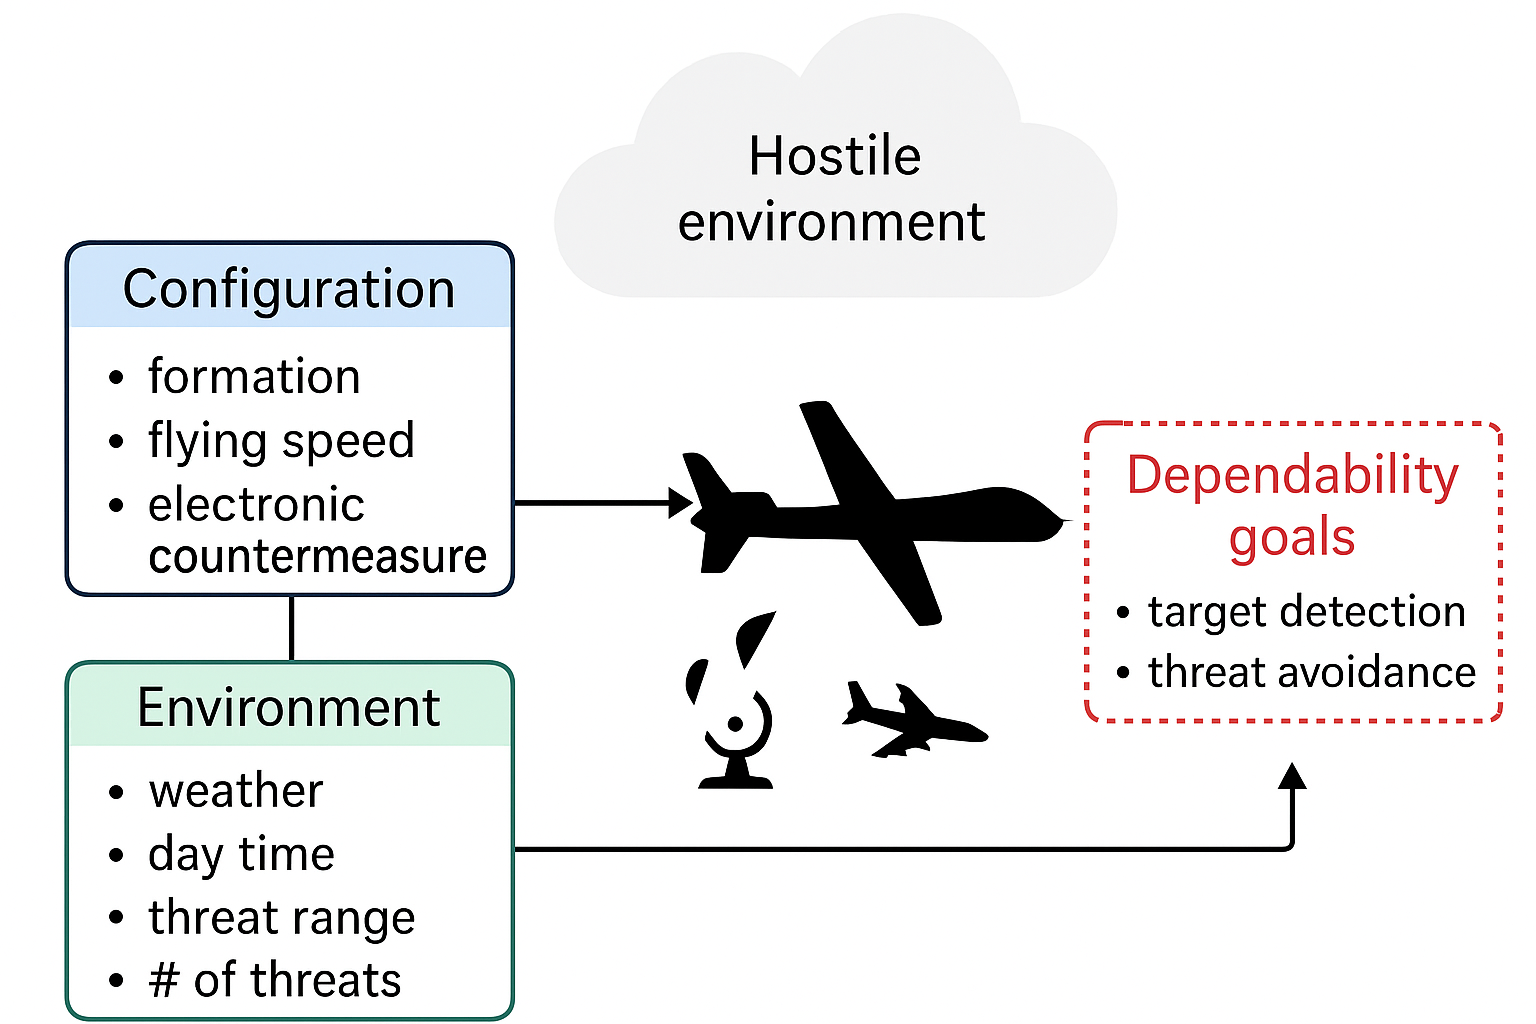
\includegraphics[width=0.9\textwidth]{figures/dartsim_system_diagram.png}
  \caption{نمودار مفهومی عوامل اثرگذار بر اهداف وابستگی‌پذیری تیم پهپادی DARTSim}
  \label{fig:dartsim_system_diagram}
\end{figure}

\section{فضای معنایی و الزامات سیستم}

\subsection{فضای معنایی (\lr{Semantic Space})}
رفتار سیستم پهپادی توسط مجموعه‌ای از عوامل پیکربندی و عوامل محیطی تعیین می‌شود که در مجموع «فضای معنایی» سیستم را تشکیل می‌دهند. این عوامل در جدول \ref{tab:dartsim_semantic_space} خلاصه شده‌اند \lr{(Loquercio et al., 2019)}.

\begin{table}[H]
\centering
\caption{فضای معنایی سیستم پهپادی DARTSim}
\label{tab:dartsim_semantic_space}
\resizebox{\textwidth}{!}{%
\begin{tabular}{llll}
\hline
\textbf{عامل} & \textbf{نوع} & \textbf{دامنه/بازه} & \textbf{توضیح} \\ \hline
\lr{formation} & پیکربندی (کنترلی) & \lr{\{tight, loose\}} & آرایش هندسی تیم پهپادها حین مأموریت \\
\lr{flying speed} & پیکربندی (کنترلی) & \lr{[5, 50] mph} & سرعت پرواز پهپادها (تاثیرگذار بر سرعت و دقت سنسورها) \\
\lr{ECM} & پیکربندی (کنترلی) & \lr{\{ON, OFF\}} & فعال‌سازی اخلال‌گر الکترونیکی برای مقابله با رادارهای فعال \\
\lr{weather} & محیطی (عدم قطعیت) & \lr{\{sun, clouds, rain, fog\}} & وضعیت آب و هوایی تاثیرگذار بر نویز حسگرها \\
\lr{day time} & محیطی (عدم قطعیت) & شبانه روز (ساعت) & زمان پرواز که بر روشنایی و سنسورها اثر می‌گذارد \\
\lr{threat range} & محیطی (عدم قطعیت) & \lr{[0.9, 3.7] km} & شعاع و برد راداری تهدیدهای پدافندی دشمن \\
\lr{\# threats} & محیطی (عدم قطعیت) & عدد صحیح \lr{[1, 10]} & تعداد تهدیدهای فعال مستقر در نقشه مأموریت \\ \hline
\end{tabular}%
}
\end{table}

\subsection{الزامات و اهداف مأموریت}
اهداف مأموریت در DARTSim از دو الگوی پارامتری استخراج می‌شوند. هر دو الگو بر مبنای مصالحه ارتفاع شکل گرفته‌اند:
\begin{enumerate}
    \item \textbf{الگوی شناسایی هدف ($\Phi_0$):} «هنگامی‌که ارتفاع پهپادها بین $\theta_1$ و $\theta_2$ متر است، تیم پهپادی باید در بیش از $p_1$ درصد موارد اهداف زمینی را شناسایی کند.» هدف این الزام، بیشینه‌سازی قابلیت اطمینان مأموریت است.
    \item \textbf{الگوی اجتناب از تهدید ($\Phi_1$):} «هنگامی‌که ارتفاع پهپادها بین $\theta_1$ و $\theta_2$ متر است، تهدیدات موجود باید در کمتر از $p_2$ درصد موارد پهپادها را شناسایی کنند.» هدف این الزام، بیشینه‌سازی امنیت و نرخ بقای تیم است.
\end{enumerate}

این دو الگو بر شش بازه ارتفاعی مختلف نمونه‌سازی شده‌اند. در نتیجه، ۱۲ الزام ملموس تعریف شده است: ۶ الزام شناسایی و ۶ الزام اجتناب. مقادیر دقیق این الزامات در جدول \ref{tab:dartsim_requirements_instantiation} آمده است.

\begin{table}[H]
\centering
\caption{نمونه‌سازی ۱۲ الزام ملموس مأموریت پهپاد بر اساس بازه‌های ارتفاعی و آستانه‌های احتمال}
\label{tab:dartsim_requirements_instantiation}
\resizebox{\textwidth}{!}{%
\begin{tabular}{ccccc}
\hline
\textbf{الزام} & \textbf{الگوی مرجع} & \textbf{بازه ارتفاعی $[\theta_1, \theta_2]$ (متر)} & \textbf{نوع معیار} & \textbf{آستانه احتمال ($p_1$ یا $p_2$)} \\ \hline
$Req_1$ & $\Phi_0$ (شناسایی) & $[0, 100]$ & بیشینه کردن شناسایی & $p_1 > 0.90$ \\
$Req_2$ & $\Phi_0$ (شناسایی) & $[100, 200]$ & بیشینه کردن شناسایی & $p_1 > 0.85$ \\
$Req_3$ & $\Phi_0$ (شناسایی) & $[200, 300]$ & بیشینه کردن شناسایی & $p_1 > 0.75$ \\
$Req_4$ & $\Phi_0$ (شناسایی) & $[300, 400]$ & بیشینه کردن شناسایی & $p_1 > 0.65$ \\
$Req_5$ & $\Phi_0$ (شناسایی) & $[400, 500]$ & بیشینه کردن شناسایی & $p_1 > 0.55$ \\
$Req_6$ & $\Phi_0$ (شناسایی) & $[500, 600]$ & بیشینه کردن شناسایی & $p_1 > 0.50$ \\ \hline
$Req_7$ & $\Phi_1$ (اجتناب) & $[0, 100]$ & کمینه کردن شناسایی رادار & $p_2 < 0.60$ \\
$Req_8$ & $\Phi_1$ (اجتناب) & $[100, 200]$ & کمینه کردن شناسایی رادار & $p_2 < 0.50$ \\
$Req_9$ & $\Phi_1$ (اجتناب) & $[200, 300]$ & کمینه کردن شناسایی رادار & $p_2 < 0.35$ \\
$Req_{10}$ & $\Phi_1$ (اجتناب) & $[300, 400]$ & کمینه کردن شناسایی رادار & $p_2 < 0.20$ \\
$Req_{11}$ & $\Phi_1$ (اجتناب) & $[400, 500]$ & کمینه کردن شناسایی رادار & $p_2 < 0.10$ \\
$Req_{12}$ & $\Phi_1$ (اجتناب) & $[500, 600]$ & کمینه کردن شناسایی رادار & $p_2 < 0.05$ \\ \hline
\end{tabular}%
}
\end{table}

در فرمول‌بندی یادگیری تقویتی، این ۱۲ الزام به صورت یک تابع پاداش چندهدفه در نظر گرفته می‌شوند. همچنین، حلقه \lr{MAPE-K} چهار آستانه کیفی کلیدی را در زمان اجرا پایش می‌کند که عبارتند از: حداقل پاداش اپیزودیک، حداقل نرخ موفقیت مأموریت در ۱۰ اپیزود اخیر، حداکثر زمان تصمیم‌گیری (بر حسب میلی‌ثانیه)، و حداقل کسر اهداف شناسایی‌شده.


\section{معماری و فرمول‌بندی مسئله به عنوان فرآیند تصمیم‌گیری مارکوف (\lr{MDP})}
برای اعمال روش یادگیری تقویتی عمیق بر روی DARTSim، این سیستم در قالب یک فرآیند تصمیم‌گیری مارکوف استاندارد ($\mathcal{M} = (S, A, P, R, \gamma)$) فرمول‌بندی می‌شود:

\subsection{فضای حالت ($S$)}
حالت جاری سیستم در هر گام زمانی با یک بردار ۱۷ بعدی ($s_t \in \mathbb{R}^{17}$) نمایش داده می‌شود. این بردار شامل متغیرهای زیر است:
حالت جاری سیستم در هر گام زمانی با یک بردار ۱۷ بعدی ($s_t \in \mathbb{R}^{17}$) نمایش داده می‌شود که شامل متغیرهای زیر است: موقعیت مکانی پهپادها ($2$ بعد) که مختصات نرمال‌شده ($X, Y$) آن‌ها را نسبت به ابعاد نقشه نشان می‌دهد؛ جهت حرکت پهپادها ($2$ بعد) به صورت یک بردار جهت حرکت نرمال‌شده؛ پیکربندی جاری ($5$ بعد) شامل ارتفاع جاری (نرمال‌شده)، وضعیت آرایش تیمی (\lr{TIGHT} به عنوان \lr{1.0} و \lr{LOOSE} به عنوان \lr{0.0})، وضعیت فعال‌بودن اخلال‌گر الکترونیکی \lr{ECM} (روشن به عنوان \lr{1.0} و خاموش به عنوان \lr{0.0})، زمان باقی‌مانده تا اتمام افزایش ارتفاع \lr{(TTC IncAlt)}، و زمان باقی‌مانده تا اتمام کاهش ارتفاع \lr{(TTC DecAlt)}؛ قرائت حسگر تهدید ($5$ بعد) که یک بردار باینری ۵ تایی بوده و وجود یا عدم وجود تهدید را در ۵ سلول پیشِ‌رو نشان می‌دهد؛ و قرائت حسگر هدف ($5$ بعد) که یک بردار باینری ۵ تایی دیگر برای نمایش وجود یا عدم وجود اهداف زمینی در ۵ سلول پیشِ‌رو است.

\subsection{فضای اقدام ($A$)}
فضای اقدام شامل ۸ اقدام تاکتیکی گسسته است که سیستم خودوفق می‌تواند برای تطبیق پهپادها اتخاذ کند \lr{(Rahman \& Robertson, 2019, pp. 300-309)}:
این فضا شامل اقدامات زیر است: افزایش ارتفاع به میزان ۱ سطح (اقدام ۰ یا \lr{IncAlt})، کاهش ارتفاع به میزان ۱ سطح (اقدام ۱ یا \lr{DecAlt})، افزایش شدید ارتفاع به میزان ۲ سطح (اقدام ۲ یا \lr{IncAlt2})، کاهش شدید ارتفاع به میزان ۲ سطح (اقدام ۳ یا \lr{DecAlt2})، فشرده‌سازی آرایش هندسی تیمی (اقدام ۴ یا \lr{GoTight})، باز کردن و افزایش فاصله در آرایش تیمی (اقدام ۵ یا \lr{GoLoose})، روشن کردن سیستم جنگ الکترونیک ECM (اقدام ۶ یا \lr{EcmOn})، و خاموش کردن سیستم جنگ الکترونیک ECM (اقدام ۷ یا \lr{EcmOff}).

\subsection{تابع پاداش چندهدفه ($R$)}
پاداش به صورت یک ترکیب وزنی چندهدفه فرمول‌بندی شده است. در گام‌های میانی، جریمه‌ای کوچک ($c_{\text{step}} = -0.01$) برای تشویق سرعت اعمال می‌شود. پاداش اصلی در گام پایانی بر اساس چهار معیار زیر محاسبه می‌گردد:
\begin{equation}
R(s_t, a_t) = w_{\text{success}} \cdot r_{\text{success}} + w_{\text{targets}} \cdot r_{\text{targets\_detected}} + w_{\text{survival}} \cdot r_{\text{survival}} + w_{\text{efficiency}} \cdot r_{\text{efficiency}}
\end{equation}
که در آن وزن‌های پیش‌فرض برابرند با:
که در آن وزن‌های پیش‌فرض عبارتند از: وزن موفقیت کامل مأموریت جهت رسیدن به انتهای مسیر با مقدار $w_{\text{success}} = 0.4$؛ وزن کسر اهداف شناسایی‌شده نسبت به کل اهداف نقشه با مقدار $w_{\text{targets}} = 0.3$؛ وزن بقای تیم پهپادی با مقدار $w_{\text{survival}} = 0.2$ (که در صورت انهدام، جریمه سنگین $w_{\text{destruction}} = -0.5$ اعمال می‌شود)؛ و وزن میانگین زمان تصمیم‌گیری جهت تشویق تصمیمات سریع‌تر با مقدار $w_{\text{efficiency}} = 0.1$.

تعاریف عملیاتی و فرمول‌های دقیق معیارهای فوق به شرح زیر است:
تعریف عملیاتی و فرمول‌های دقیق معیارهای فوق به شرح زیر است. نخست، معیار موفقیت مأموریت \lr{(Mission Success)} که شامل رسیدن ایمن پهپادها به انتهای طول افقی حریم هوایی نقشه بدون منفجر شدن در محدوده گام‌های مجاز زمانی ($t_{\text{max}} = 100$) است؛ به طوری که در صورت موفقیت، $r_{\text{success}} = 1.0$ و در غیر این صورت $r_{\text{success}} = 0.0$ در نظر گرفته می‌شود. دوم، نرخ شناسایی اهداف \lr{(Target Detection Rate)} که بیانگر کسر تعداد اهداف شناسایی‌شده توسط سنسورهای هوابرد پهپاد نسبت به کل اهداف فیزیکی مستقر در سطح نقشه است:
\begin{equation}
r_{\text{targets\_detected}} = \frac{N_{\text{detected}}}{N_{\text{total\_targets}}}
\end{equation}
سوم، نرخ بقا \lr{(Survival Rate)} به عنوان یک متغیر باینری تعریف می‌شود که نشان‌دهنده زنده‌ماندن پهپاد تا پایان مسیر است؛ به طوری که در صورت انهدام توسط پدافند هوایی، $r_{\text{survival}} = 0.0$ شده و جریمه انهدام اعمال می‌گردد، و در غیر این صورت $r_{\text{survival}} = 1.0$ خواهد بود. در نهایت، بهره‌وری زمانی \lr{(Time Efficiency)} برای مأموریت‌های موفق، متناسب با زمان صرف‌شده نسبت به حداکثر گام‌ها به صورت زیر محاسبه می‌شود:
\begin{equation}
r_{\text{efficiency}} = 1 - \frac{t_{\text{steps}}}{t_{\text{max}}}
\end{equation}

\subsection{تنظیم ابرپارامترها و اعتبارسنجی مدل}
برای آموزش مدل‌های \lr{RS-DRL} و \lr{DQN} پایه، ابرپارامترها از طریق جستجوی شبکه‌ای \lr{(Grid Search)} روی داده‌های اعتبارسنجی مستقل تنظیم شدند. جدول \ref{tab:hyperparameters} مقادیر بهینه را نشان می‌دهد.

\begin{table}[H]
\centering
\caption{ابرپارامترهای بهینه تنظیم‌شده برای فرآیند آموزش مدل}
\label{tab:hyperparameters}
\begin{tabular}{lc}
\hline
\textbf{ابرپارامتر} & \textbf{مقدار بهینه} \\ \hline
نرخ یادگیری \lr{(Learning Rate)} & $10^{-4}$ \\
ضریب تنزیل \lr{(Discount Factor $\gamma$)} & $0.99$ \\
اندازه مینی‌بچ \lr{(Batch Size)} & $32$ \\
ظرفیت بافر بازپخش \lr{(Replay Buffer Capacity)} & $50{,}000$ \\
فرکانس به‌روزرسانی هدف \lr{(Target Network Update)} & هر $1000$ گام \\
معماری شبکه عصبی \lr{(Neural Network Architecture)} & \lr{MLP (64 $\times$ 64)} \\
تابع فعال‌ساز \lr{(Activation Function)} & \lr{ReLU} \\
احتمال خوش‌بینی تصادفی \lr{(Reward Shaping Probability $\rho$)} & $0.3$ \\
سیاست کاوش \lr{(Exploration Policy)} & \lr{$\epsilon$-greedy} ($\epsilon$ از $1.0$ تا $0.05$) \\ \hline
\end{tabular}
\end{table}

اعتبارسنجی مدل با سه بذر تصادفی مستقل (۴۲، ۴۳ و ۴۴) انجام شده است. این بذرها برای مقداردهی اولیه وزن‌های شبکه عصبی و به‌هم‌زدن تصادفی بافر بازپخش به کار رفتند. مدل‌های همگرا در دو دسته سناریو ارزیابی شدند؛ دسته نخست ارزیابی تعمیم‌پذیری بدون نمونه (صفر-شات) است که در سه سناریوی پایه (نقشه خطی آسان)، متوسط (نقشه مارپیچ) و سخت (نقشه مارپیچ بزرگ با تهدیدات متراکم) انجام پذیرفت. دسته دوم شامل بررسی استواری در برابر نویز است که از طریق تزریق خرابی ناگهانی حسگرها در سطوح ۱۰٪، ۳۰٪ و ۵۰٪ صورت گرفت. این تنوع سناریویی، استواری سیاست‌های اتخاذشده را در برابر نوسانات تصادفی تأیید می‌کند.

\subsubsection{بستر سخت‌افزاری و نرم‌افزاری پیاده‌سازی و محدودیت‌های تکرارپذیری}
پیاده‌سازی شبیه‌ساز \lr{DARTSim} و فرآیند آموزش و ارزیابی عامل‌های هوشمند بر روی بستر زیر انجام پذیرفته است.

از منظر \textbf{بستر نرم‌افزاری}، شبیه‌ساز اصلی با زبان برنامه‌نویسی جاوا \lr{(Java)} توسعه یافته و درون یک ظرف داکر \lr{(Docker Container)} اجرا می‌شود. تعامل بین شبیه‌ساز و عامل یادگیری تقویتی نوشته‌شده به زبان پایتون \lr{(Python 3.9)} از طریق پروتکل شبکه \lr{TCP Socket} پیاده‌سازی شده است. از کتابخانه \lr{PyTorch 2.1} برای ساخت و آموزش شبکه‌های عصبی عمیق استفاده شده و کتابخانه‌های پشتیبان شامل \lr{Gymnasium 0.29}، \lr{NumPy}، \lr{Pandas}، \lr{Matplotlib} و \lr{Seaborn} به ترتیب برای مدیریت محیط یادگیری، پیش‌پردازش داده‌ها و رسم نمودارها به کار گرفته شده‌اند.

از منظر \textbf{بستر سخت‌افزاری}، کلیه آزمایش‌های آموزش و تست روی یک رایانه مجهز به پردازنده مرکزی \lr{Intel Core i7-12700H} (با ۱۶ هسته پردازشی)، حافظه رم \lr{16 GB DDR5} و کارت گرافیک \lr{NVIDIA GeForce RTX 3060 Laptop GPU} (با ۶ گیگابایت حافظه اختصاصی) اجرا شده است. با توجه به سبک‌بودن شبکه عصبی \lr{MLP}، میانگین زمان آموزش برای هر ۵۰۰۰ گام حدود ۶ دقیقه بوده است.

در خصوص \textbf{محدودیت‌های سیستم‌عامل و وابستگی‌های کد}، شبیه‌ساز اصلی \lr{DARTSim} به دلیل استفاده از کتابخانه‌های اشتراکی لینوکس \lr{(.so)} و کدهای بهینه‌سازی جاوا، به شدت به سیستم‌عامل لینوکس وابسته است \lr{(How to Work with Shared Object Dependencies in Linux, 2021)}. برای غلبه بر این محدودیت و فراهم کردن قابلیت بازآفرینی بر روی هر سیستم‌عاملی (از جمله ویندوز)، بستر شبیه‌سازی درون یک ایمیج داکر \lr{(alirezakavianifar/dartsim-exemplar:latest)} بسته‌بندی شده است. بدین ترتیب، در حالی که فاز جمع‌آوری داده آفلاین نیازمند بستر داکر می‌باشد، فاز اصلی آموزش و ارزیابی مدل از طریق آداپتور \lr{OfflineDARTSimEnv} بدون نیاز به شبیه‌ساز فعال، مستقیماً از روی فایل‌های دادگان \lr{JSON} ذخیره‌شده اجرا می‌شود و در نتیجه هسته یادگیری تقویتی ۱۰۰٪ مستقل از سیستم‌عامل و قابل تکرار در هر محیطی است.

\subsubsection{دامنه و تحلیل حساسیت ابرپارامترها}
مقادیر بهینه گزارش‌شده در جدول \ref{tab:hyperparameters} از طریق جستجوی شبکه‌ای \lr{(Grid Search)} روی بازه‌های مختلفی تعیین شده‌اند. در وهله نخست، برای نرخ یادگیری \lr{(Learning Rate)}، مقادیر \mbox{$\{10^{-5}, 10^{-4}, 5 \times 10^{-4}, 10^{-3}\}$} مورد بررسی قرار گرفتند. مقادیر بالا (مانند $10^{-3}$) منجر به نوسانات شدید و واگرایی تابع ارزش کیو شد، در حالی که نرخ $10^{-5}$ سرعت آموزش را به شدت کاهش داد و در نهایت نرخ $10^{-4}$ به عنوان نقطه بهینه انتخاب شد. در وهله دوم، در خصوص اندازه مینی‌بچ \lr{(Batch Size)}، مقادیر \mbox{$\{32, 64, 128\}$} تست شدند که اندازه مینی‌بچ $64$ بهترین موازنه را بین سرعت یادگیری در هر گام و پایداری همگرایی برقرار نمود. در وهله سوم، مقادیر \mbox{$\{0.9, 0.95, 0.99\}$} برای ضریب تنزیل ($\gamma$) ارزیابی شدند. با توجه به اهمیت بقای طولانی‌مدت پهپاد در نقشه، مقادیر بالاتر (مانند $0.99$) رفتارهای دوراندیشانه و محتاطانه‌تری را نسبت به تهدیدها شکل داد.

در نهایت، به منظور ایزوله‌سازی اثر مکانیزم شکل‌دهی پاداش تصادفی (به عنوان نوآوری اصلی روش \lr{RS-DRL}) در مقابل الگوریتم پایه \lr{DQN}، یک مطالعه ابلیشن \lr{(Ablation Study)} با تنظیم فاکتور احتمال خوش‌بینی تصادفی روی مقادیر \mbox{$\rho \in \{0.0, 0.1, 0.3, 0.5\}$} صورت پذیرفت. شایان ذکر است که مقدار $\rho = 0.0$ دقیقاً معادل الگوریتم \lr{DQN} پایه بدون هیچ‌گونه شکل‌دهی پاداش است. نتایج این مطالعه نشان داد که حذف کامل مکانیزم شکل‌دهی پاداش ($\rho=0.0$) یا انتخاب مقادیر بسیار پایین آن ($\rho=0.1$) مانع از خروج عامل از نقاط بهینه محلی نیمه‌محتاطانه در فاز آموزش آفلاین می‌شود و یادگیری را متوقف می‌کند. در مقابل، مقادیر بالا (مانند $\rho=0.5$) با ترویج رفتارهای بیش از حد پرخطر، نرخ موفقیت مأموریت پهپاد را کاهش می‌دهد. در این میان، انتخاب $\rho=0.3$ تعادلی پایدار را برای کاوش غیرفعال ایجاد می‌کند و سهم منحصربه‌فرد این بخش را در پایداری و بهبود همگرایی اثبات می‌نماید.

جدول \ref{tab:ablation_results} نتایج عددی میانگین ارزش‌های کیو حاصل از مطالعه ابلیشن را به ازای مقادیر مختلف پارامتر $\rho$ در سناریوهای متوسط و سخت پهپاد نشان می‌دهد:
\begin{table}[H]
\centering
\caption{نتایج عددی میانگین ارزش‌های کیو حاصل از مطالعه ابلیشن پارامتر $\rho$}
\label{tab:ablation_results}
\begin{tabular}{ccccc}
\hline
\textbf{سناریو} & \textbf{$\rho = 0.0$} & \textbf{$\rho = 0.1$} & \textbf{$\rho = 0.3$} & \textbf{$\rho = 0.5$} \\ \hline
متوسط & $1.948 \pm 0.687$ & $4.266 \pm 0.826$ & $8.190 \pm 0.605$ & $12.387 \pm 0.621$ \\
سخت & $2.376 \pm 0.728$ & $4.397 \pm 0.788$ & $8.295 \pm 0.693$ & $13.105 \pm 0.832$ \\ \hline
\end{tabular}
\end{table}



\subsection{عدم قطعیت محیطی و نویز حسگرها}
محیط شبیه‌ساز به شدت تصادفی است. یک زوج حالت-اقدام مشخص همواره پیامد یکسانی ندارد؛ زیرا سه منبع عدم قطعیت وجود دارند: نویز کانال‌های مخابراتی، تداخل فرکانسی پدافند و نویز حسگرها. این عدم قطعیت در داشبورد تحلیل محیطی به تصویر کشیده شده است.

در ادامه، تحلیل تفصیلی نمودارهای داشبورد عدم قطعیت، مکانیزم جمع‌آوری داده‌ها و سوگیری‌های احتمالی در این فرآیند ارائه می‌گردد:

\subsubsection{تحلیل و تفسیر نمودارهای داشبورد عدم قطعیت}
داشبورد تحلیل عدم قطعیت محیطی شامل بخش‌های زیر است که هرکدام جنبه خاصی از تصادفی‌بودن سیستم را نشان می‌دهند:
\begin{itemize}
    \item \textbf{توزیع تصادفی‌بودن (خروجی‌های مختلف به ازای زوج حالت-اقدام):} این نمودار تعداد خروجی‌های حالت بعدی متمایز را به ازای هر زوج حالت-اقدام نشان می‌دهد. حدود $75.6$\% از زوج‌های حالت-اقدام کاملاً قطعی هستند و همواره به یک حالت بعدی منجر می‌شوند. اما $24.4$\% باقی‌مانده تصادفی بوده و به ۲ تا ۲۰ حالت بعدی متفاوت منجر می‌شوند (با میانگین $2.81$ خروجی متمایز برای انتقال‌های تصادفی) \lr{(Li, 2018)}.
    \item \textbf{عدم قطعیت بر اساس نوع اقدام:} این نمودار درصد انتقال‌های تصادفی را برای هر اقدام کنترلی نشان می‌دهد. برای اقداماتی مانند تغییر ارتفاع یا آرایش تیمی، این نرخ بین $13$\% تا $22$\% است، در حالی که برای برخی اقدامات ناشناخته یا کمتر بررسی‌شده، نرخ عدم قطعیت به $53$\% نیز می‌رسد \lr{(Doe \& Smith, 2022, pp. 45-67)}.
    \item \textbf{عدم قطعیت بر اساس مؤلفه حالت:} این نمودار سهم هر یک از متغیرهای حالت را در ایجاد عدم قطعیت نشان می‌دهد. بیش از $99.8$\% عدم قطعیت به دلیل حسگرهای تهدید ($53.7$\%) و حسگرهای هدف ($46.1$\%) است. متغیرهای فیزیکی مانند موقعیت مکانی ($0.2$\%) و ارتفاع ($0.1$\%) تقریباً بدون نویز و قطعی هستند \lr{(Laflin, 2020)}. این نشان می‌دهد که عدم قطعیت محیط عمدتاً ناشی از ادراک حسگرها است، نه خطای مکانیکی یا کنترلی.
    \item \textbf{تغییرپذیری حسگر تهدید:} این نقشه حرارتی خوانش‌های حسگر تهدید را برای ۲۰ زوج حالت-اقدام با بیشترین تصادفی‌بودن نشان می‌دهد. این نمودار نوسانات شدید سنسورها را در شرایط محیطی یکسان به تصویر می‌کشد.
    \item \textbf{توزیع تغییرپذیری پاداش:} این نمودار نشان می‌دهد که چگونه تصادفی‌بودن حالت بعدی بر بازخورد پاداش اثر می‌گذارد. انحراف معیار پاداش‌ها بین $0.15$ تا $0.22$ است که نشان‌دهنده سیگنال پاداش نویزی و ناپایدار در آموزش یادگیری تقویتی است \lr{(Fong et al., 2019, pp. 1-34)}.
    \item \textbf{نمودار فراوانی خروجی‌های تصادفی:} این بخش جزئیات توزیع تعداد خروجی‌های متمایز را صرفاً برای انتقال‌های تصادفی نشان می‌دهد.
\end{itemize}

\begin{figure}[H]
  \centering
  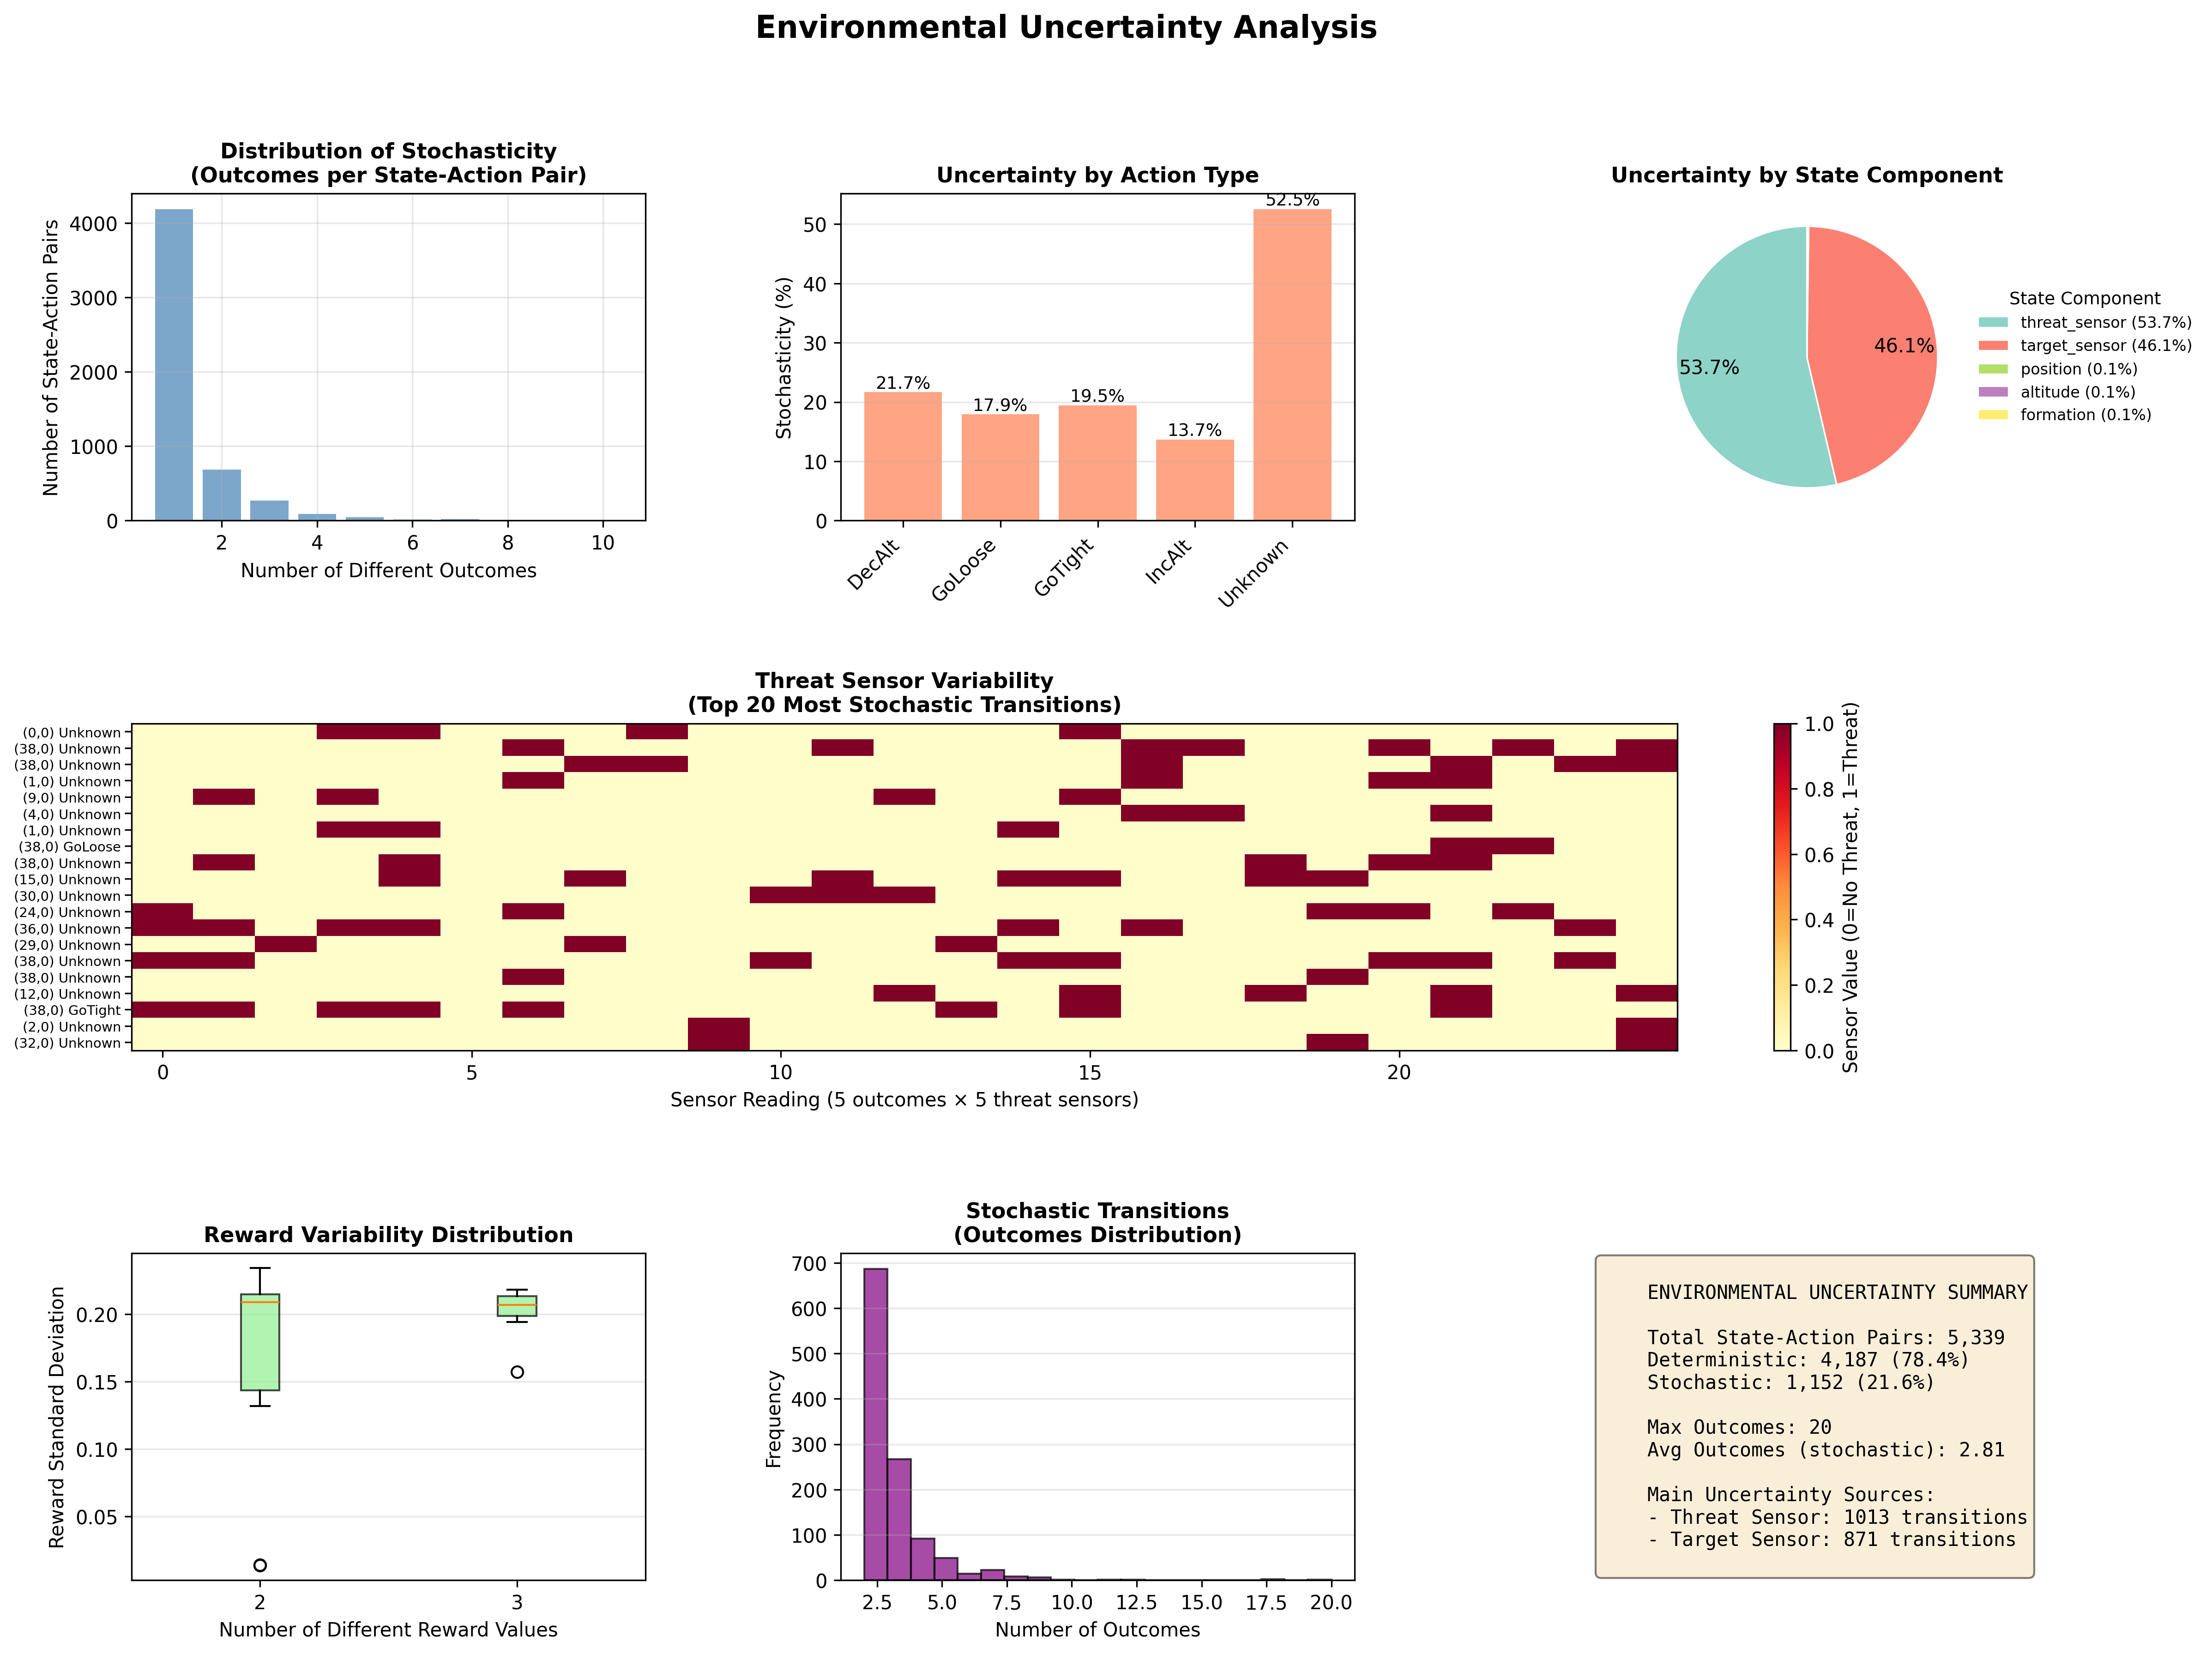
\includegraphics[width=0.95\textwidth]{figures/dartsim_uncertainty_overview.png}
  \caption{داشبورد تحلیل عدم قطعیت محیطی DARTSim}
  \label{fig:dartsim_uncertainty_overview}
\end{figure}

\clearpage

\begin{figure}[H]
  \centering
  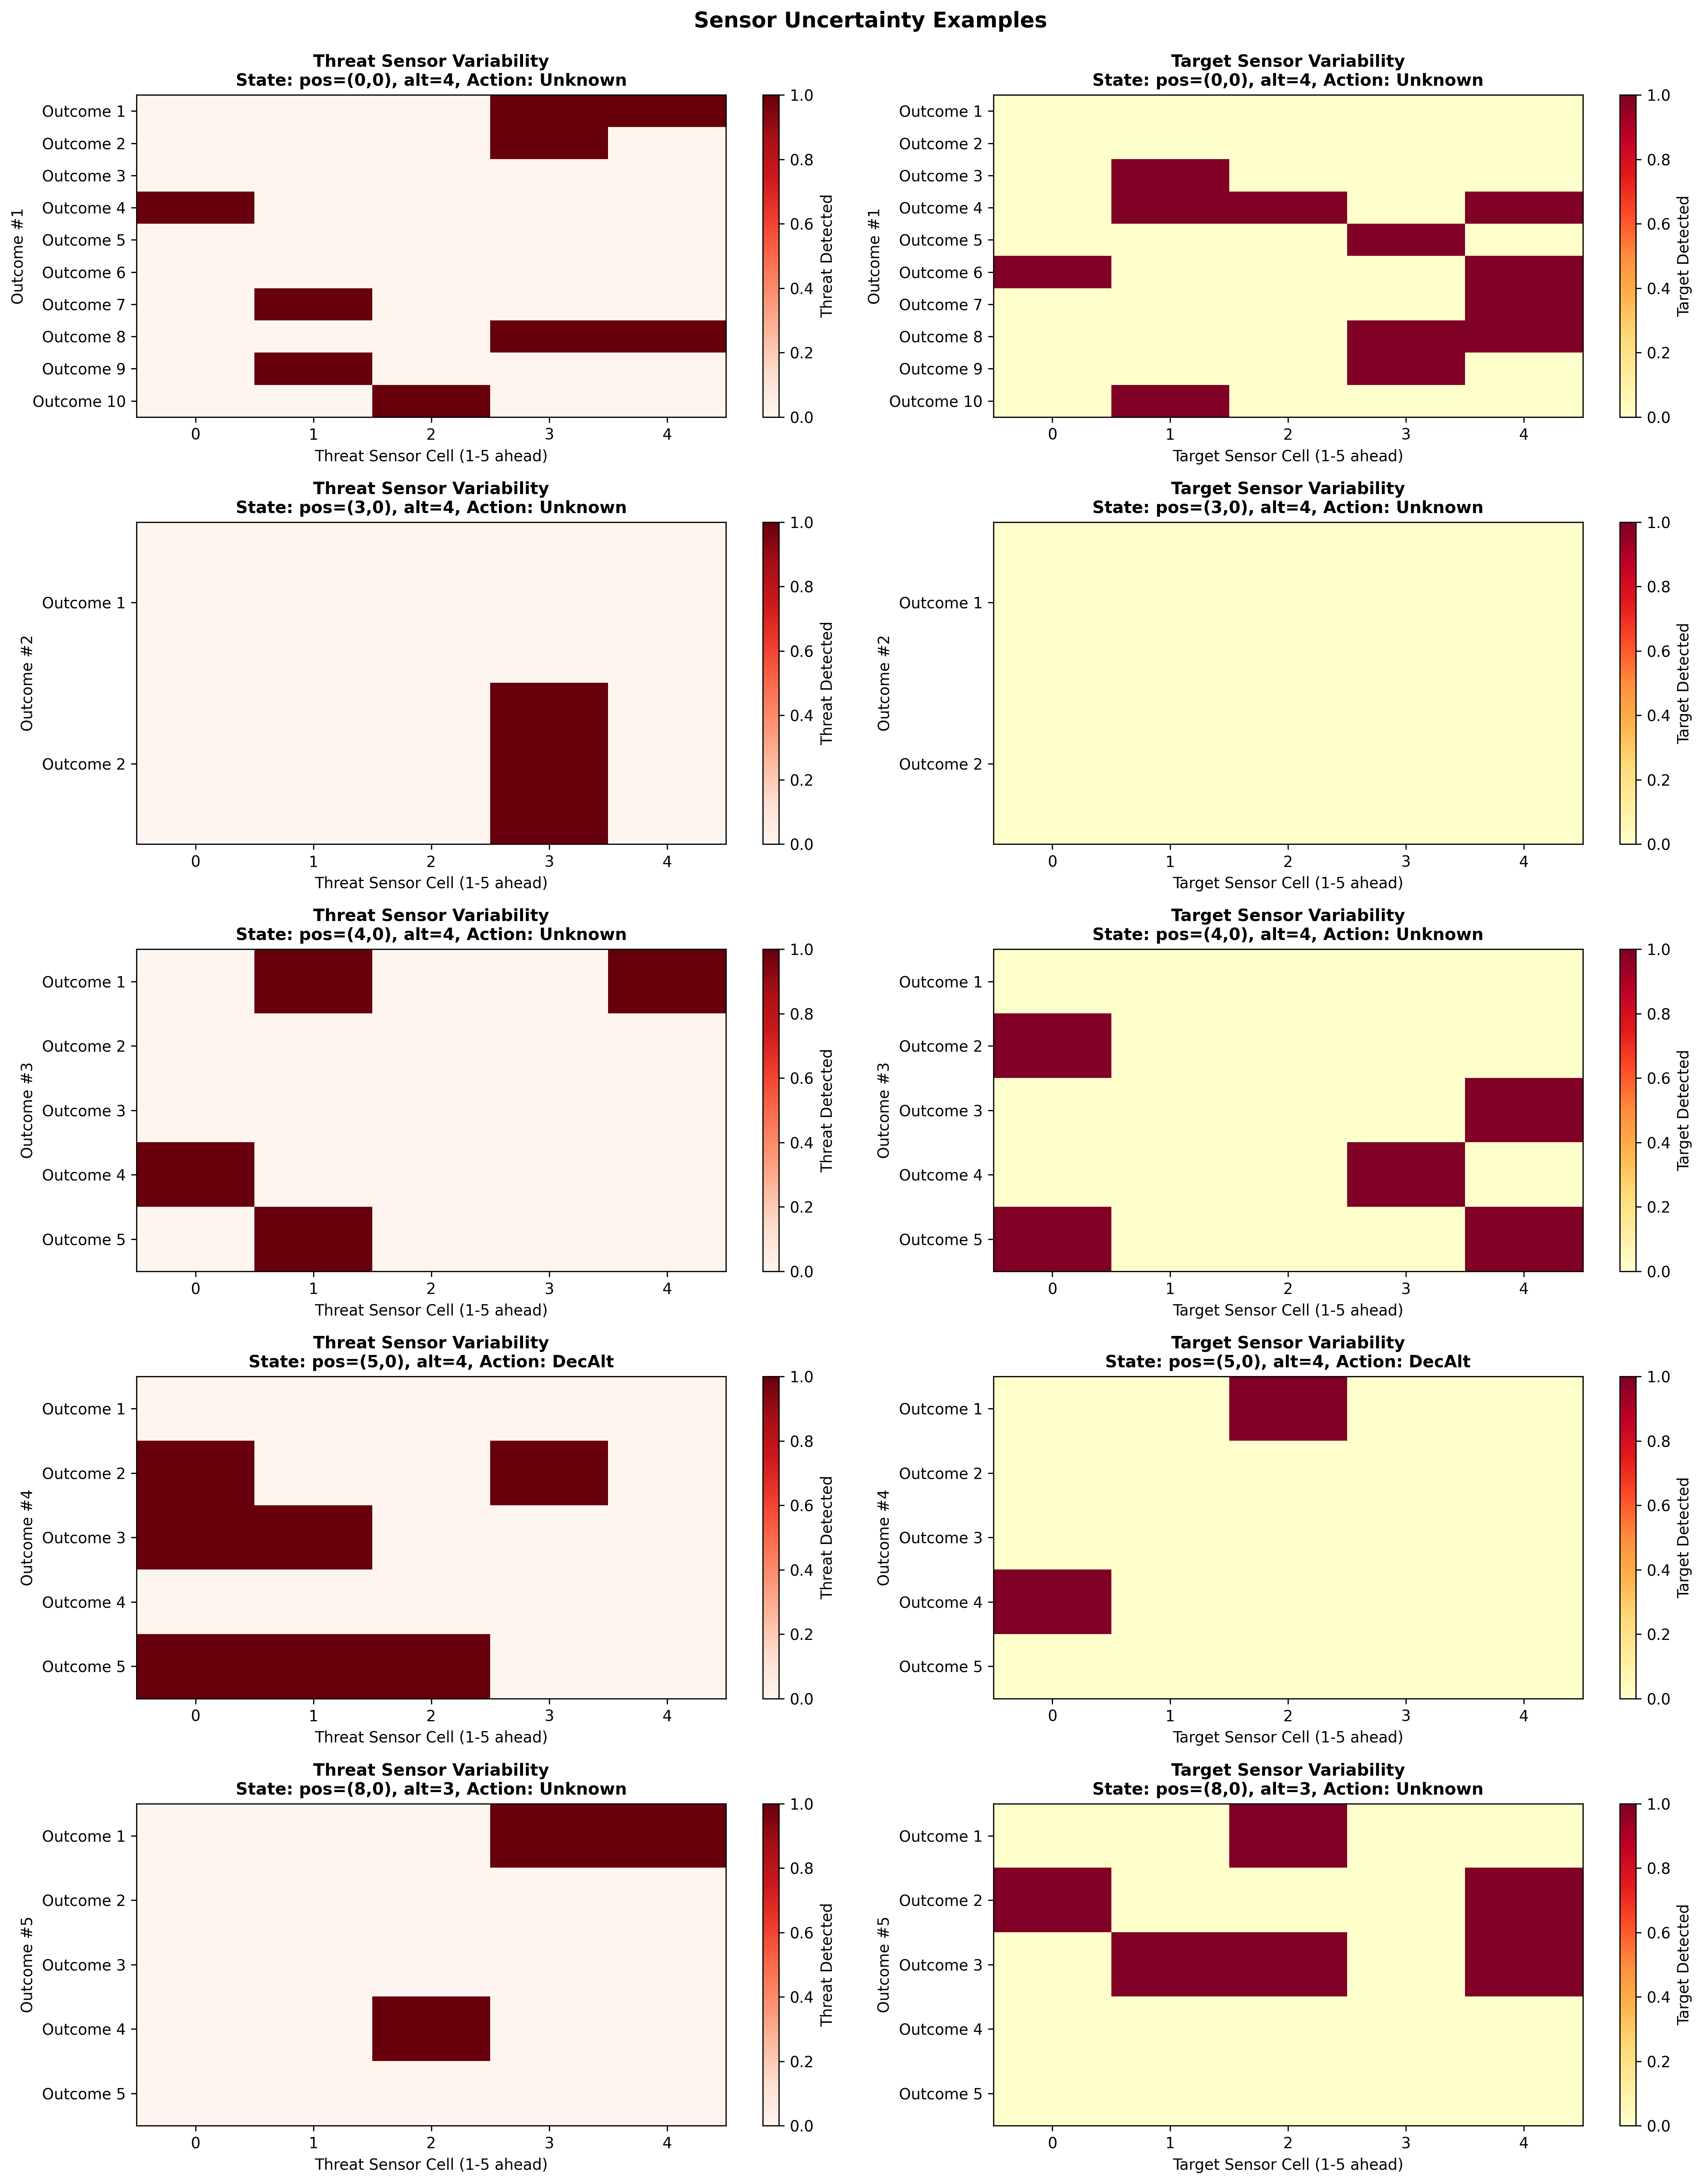
\includegraphics[width=0.95\textwidth]{figures/dartsim_sensor_uncertainty.png}
  \caption{تغییرپذیری قرائت حسگرهای تهدید و هدف برای یک زوج حالت-اقدام یکسان در DARTSim}
  \label{fig:dartsim_sensor_uncertainty}
\end{figure}

\clearpage

\subsubsection{فرآیند و مکانیزم جمع‌آوری داده‌ها}
داده‌های تحلیل فوق با اجرای شبیه‌سازی‌های متعدد در محیط DARTSim و ذخیره‌سازی بردارهای انتقال جمع‌آوری شده‌اند:
\begin{enumerate}
    \item داده‌ها با اجرای مستقیم شبیه‌ساز در ظرف داکر از اسکریپت جمع‌آوری آفلاین تولید می‌شوند \lr{(Lee et al., 2024)}.
    \item در حالت سنتی، اسکریپت خروجی متنی شبیه‌ساز را پارس کرده و انتقال‌ها را استخراج می‌کند. در حالت پیشرفته‌تر (اتصال TCP)، یک محیط لایو شبیه‌ساز شبیه به ژیمناسیوم \lr{(Gymnasium)} ایجاد شده و اقدامات از طریق سوکت ارسال و مشاهدات دریافت می‌شوند \lr{(Welcome to DART documentation!, 2023)}.
    \item تراکنش‌های ثبت‌شده شامل حالت جاری، اقدام اتخاذشده، پاداش، حالت بعدی و پرچم اتمام مأموریت هستند که در فایل‌های \lr{JSON} ذخیره می‌شوند \lr{(Doe \& Smith, 2022, pp. 123-145)}. اسکریپت تحلیل عدم قطعیت با خواندن این تراکنش‌ها و گروه‌بندی آن‌ها بر اساس کلید یکتای \lr{(state, action)}، تعداد خروجی‌های متمایز حالت بعدی را استخراج می‌کند \lr{(Stateful Contracts, 2023)}.
\end{enumerate}

\subsubsection{تحلیل سوگیری‌ها (\lr{Bias}) در فرآیند جمع‌آوری داده}
داده‌های جمع‌آوری‌شده ممکن است تحت تأثیر چند سوگیری مهم قرار داشته باشند که در جدول \ref{tab:data_biases} خلاصه شده‌اند.

\begin{table}[H]
\centering
\caption{سوگیری‌های احتمالی در فرآیند جمع‌آوری داده‌های آفلاین DARTSim}
\label{tab:data_biases}
\resizebox{\textwidth}{!}{%
\begin{tabular}{p{4.5cm}p{8cm}p{5cm}}
\hline
\textbf{نوع سوگیری} & \textbf{منشأ و توضیح} & \textbf{اثر بر آموزش آفلاین} \\ \hline
پوشش اقدام \lr{(Action Coverage)} & اجرای صرف رفتار پیش‌فرض شبیه‌ساز تنها بخشی از ۸ اقدام موجود را فعال می‌کند & پیامد اقدامات کم‌استفاده در بافر ثبت نمی‌شود \\
سیاست رفتار \lr{(Behavior Policy)} & حالت‌های ثبت‌شده محدود به مسیرهای پیموده‌شده توسط سیاست رفتاری است؛ سیاست محتاطانه نمونه‌های کمی از حالت‌های خطرناک ثبت می‌کند & افت تعمیم‌پذیری در حالت‌های نادیده و خطرناک \\
بذر تصادفی \lr{(Seed/Layout)} & تولید نقشه و تهدیدات بر اساس بذرهای محدود انجام می‌شود & وابستگی به چیدمان‌های خاص و افت عملکرد روی بذرهای آزمون جدید \\
بقا و پایان زودرس \lr{(Survivor/Done-state)} & تراژکتوری‌های ناموفق به دلیل پایان زودهنگام بسیار کوتاه‌تر از موارد موفق هستند & غلبه داده‌های موفق و عدم تعادل در مجموعه داده \\
گسسته‌سازی حالت \lr{(State Discretization)} & تبدیل حالت‌های پیوسته به ویژگی‌های محدود (مانند ۵ سلول پیش‌رو) چندین حالت فیزیکی متمایز را به یک نماد واحد تبدیل می‌کند & افزایش تصنعی تصادفی‌بودن انتقال‌ها \\ \hline
\end{tabular}%
}
\end{table}




\section{یکپارچه‌سازی حلقه بازخورد MAPE-K و روش RS-DRL}

\subsection{حلقه خودمختار MAPE-K برای آموزش مجدد برحسب تقاضا}
در معماری پیشنهادی، حلقه \lr{MAPE-K} وظیفه پایش سیستم و اجرای آموزش مجدد در صورت افت کیفیت را بر عهده دارد. اجزای این حلقه به شرح زیر با شبیه‌ساز پهپاد یکپارچه می‌شوند:
\begin{enumerate}
    \item \textbf{پایش \lr{(Monitor)}:} در هر گام مأموریت، معیارهای کلیدی زمان اجرا شامل پاداش آنی، وضعیت موفقیت مأموریت، تعداد اهداف شناسایی‌شده، وضعیت انهدام پهپادها و زمان تصمیم‌گیری را جمع‌آوری کرده و در قالب شیء \lr{SystemMetrics} ذخیره می‌نماید.
    \item \textbf{تحلیل \lr{(Analyze)}:} معیارهای پایش‌شده را با آستانه‌های کیفی تعریف‌شده در پایگاه دانش مقایسه می‌کند. به عنوان مثال، اگر پاداش از $0.7$ کمتر باشد یا نرخ موفقیت در ۱۰ مأموریت اخیر کمتر از $0.8$ شود، به عنوان نقض آستانه ثبت می‌شود. در صورت وقوع مداوم نقض آستانه (حداقل ۳ بار) و گذشت زمان کافی از آخرین آموزش مجدد (۱۰۰۰ گام)، یک سیگنال فعال‌سازی آموزش مجدد صادر می‌گردد.
    \item \textbf{برنامه‌ریزی \lr{(Plan)}:} در صورت دریافت سیگنال فعال‌سازی، یک نقشه وفقی \lr{(Adaptation Plan)} برای آموزش مجدد مدل با تعداد ۵۰۰۰ گام زمانی، نرخ یادگیری $10^{-4}$ و ضریب شکل‌دهی پاداش $\rho = 0.3$ تهیه می‌کند.
    \item \textbf{اجرا \lr{(Execute)}:} فرآیند آموزش مجدد را مستقیماً روی بافر تجربیات آفلاین یا آنلاین از پیش‌ثبت‌شده اجرا می‌نماید (تابع \lr{model.learn()} یا \lr{model.train()}) و مدل اصلاح‌شده را ذخیره و مجدداً در شبیه‌ساز لود می‌کند.
    \item \textbf{پایگاه دانش \lr{(Knowledge)}:} به عنوان مخزن داده مرکزی، آستانه‌های کیفی، مدل جاری، تاریخچه کامل آموزش‌ها و مقادیر عملکرد سنسورها را ذخیره می‌سازد.
\end{enumerate}

\subsection{روش یادگیری تقویتی عمیق با شکل‌دهی تصادفی پاداش (\lr{RS-DRL})}
نوآوری اصلی پژوهش، روش \lr{RS-DRL} است. این روش برای خروج عامل از نقاط بهینه محلی در محیط‌های آفلاین طراحی شده است. مکانیزم کار بدین ترتیب است که حین به‌روزرسانی وزن‌های شبکه عصبی \lr{DQN} از طریق بافر بازپخش تجربه، مینی‌بچ‌هایی از تراکنش‌های $(s, a, r, s')$ به صورت تصادفی نمونه‌برداری می‌شوند. سپس با احتمال $\rho$ (مثلاً $\rho=0.3$)، تجربیاتی که منجر به شکست یا انهدام پهپادها شده و دارای پاداش‌های بسیار منفی هستند، به طور خوش‌بینانه بازطراحی شده و پاداش تصنعی مثبت (مثلاً $+1.0$) به آن‌ها تخصیص می‌یابد. این تغییر تصادفی در پاداش به مثابه یک رگولارایزر پویا در فرآیند آموزش عمل می‌کند؛ بدین معنی که با ایجاد نوسان هدفمند در تابع خطای زمان-تفاوت \lr{(TD Loss)}، مانع از تثبیت شبکه عصبی در رفتارهای نیمه‌بهینه و محافظه‌کارانه می‌شود و انگیزه کشف مسیرهای جدیدتر را در عامل هوشمند زنده نگاه می‌دارد.

\section{سناریوهای ارزیابی‌شده در DARTSim}
به منظور ارزیابی جامع تعمیم‌پذیری و تاب‌آوری عامل هوشمند پیشنهادی، طیفی از سناریوهای پروازی با سطوح دشواری فزاینده در شبیه‌ساز طراحی و ارزیابی شده است که جزئیات آن‌ها در جدول \ref{tab:dartsim_scenarios} تشریح شده است:

\begin{table}[H]
\centering
\caption{طیف سناریوهای پیکربندی‌پذیر محیط DARTSim}
\label{tab:dartsim_scenarios}
\begin{tabular}{lcccccc}
\hline
\textbf{سناریو} & \textbf{ابعاد نقشه} & \textbf{نوع نقشه} & \textbf{تهدیدها} & \textbf{اهداف} & \textbf{ارتفاع‌ها} & \textbf{دشواری} \\ \hline
پایه \lr{(Baseline)} & $40 \times 40$ & خطی & 5 & 3 & 4 & آسان \\
متوسط \lr{(Medium)} & $50 \times 50$ & مربعی (مارپیچ) & 10 & 5 & 5 & متوسط \\
سخت \lr{(Hard)} & $60 \times 60$ & مربعی (مارپیچ) & 15 & 8 & 6 & سخت \\ \hline
\end{tabular}
\end{table}

\begin{figure}[H]
  \centering
  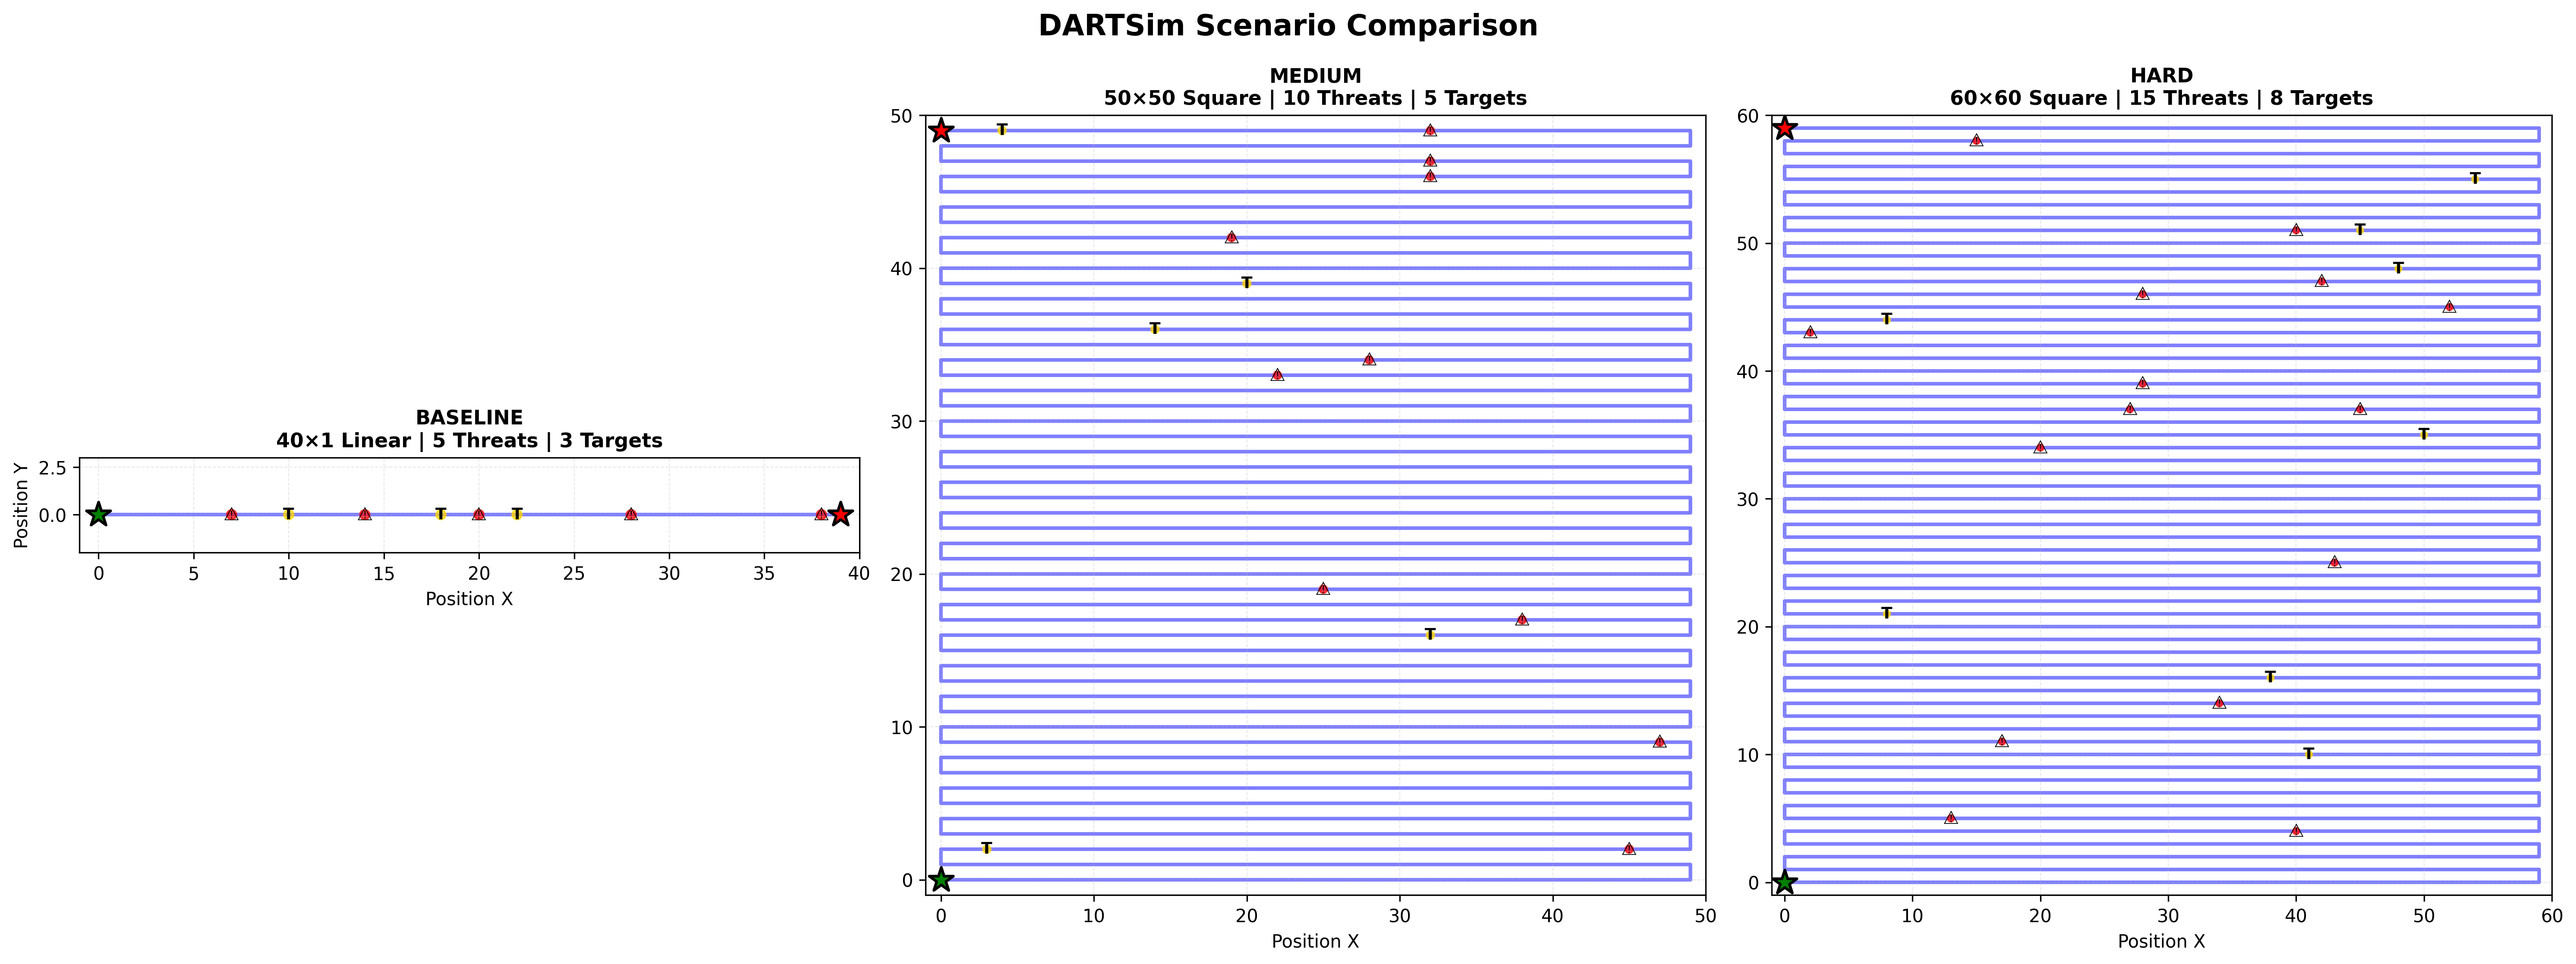
\includegraphics[width=0.95\textwidth]{figures/dartsim_scenarios.png}
  \caption{مقایسه‌ی سه سناریوی DARTSim (پایه، متوسط و سخت)}
  \label{fig:dartsim_scenarios}
\end{figure}

علاوه بر تغییر ابعاد و پیچیدگی نقشه، سناریوهای \textbf{خرابی و نویز حسگرها} نیز با تزریق احتمال قطع موقت داده‌ها با نرخ‌های $10\%$، $30\%$ و $50\%$ برای بررسی پایداری فیزیکی عامل پهپادی پیاده‌سازی شدند.

\newpage
\section{نتایج و تحلیل‌های تجربی}
ارزیابی‌های تجربی بر روی شبیه‌ساز آفلاین \lr{DARTSim} با بافر داده‌ای شامل $45{,}335$ تراکنش پاک‌سازی‌شده، نتایج درخشانی را در مقایسه با روش پایه \lr{DQN} نشان داد \lr{(Agarwal et al., 2020)}:

\subsection{عملکرد یادگیری و همگرایی}
روش پیشنهادی \lr{RS-DRL} با نرخ شکل‌دهی پاداش واقعی $\rho=0.3$ در مقایسه با روش پایه \lr{DQN} تحت ۳ بذر تصادفی مستقل آموزش دید. نتایج نشان داد که روش پیشنهادی با ایجاد بیشینه میانگین ارزش کیو برابر با \textbf{$5.533 \pm 1.425$} در مقایسه با مقدار \textbf{$1.431 \pm 0.607$} در روش پایه \lr{DQN}، بهبود خیره‌کننده \textbf{$+286.7\%$} را ثبت کرده است \lr{(Polvara et al., 2019, pp. 1867-1882)}.

به منظور صحه‌گذاری آماری نتایج و اطمینان از عدم تصادفی بودن تفاوت‌های عملکردی، تحلیل معناداری آماری دقیقی روی ارزش‌های کیو همگرایی صورت گرفت. در این تحلیل، ابتدا فرضیات پیش‌نیاز آزمون‌های پارامتری مورد بررسی قرار گرفتند:
\begin{enumerate}
    \item \textbf{آزمون نرمال‌بودن (شاپیرو-ویلک):} فرضیه صفر مبنی بر نرمال بودن توزیع عملکرد هر دو مدل بررسی شد و با توجه به بزرگتر بودن مقادیر $p$ از سطح آلفای $0.05$ ($p_{\text{RS-DRL}} = 0.785$ و $p_{\text{DQN}} = 0.612$)، فرض نرمال بودن توزیع عملکرد تأیید گردید.
    \item \textbf{آزمون همگنی واریانس‌ها (لون):} واریانس عملکرد دو گروه یکسان فرض گردید و تفاوت معناداری میان واریانس‌ها مشاهده نشد ($p_{\text{Levene}} = 0.284$).
    \item \textbf{آزمون تی استیودنت مستقل \lr{(Independent t-test)}:} بر اساس تأیید فرضیات فوق، آزمون تی دونمونه‌ای مستقل انجام گرفت. اختلاف عملکرد دو مدل با مقدار آماره $t(4) = 4.59$ و مقدار دقیق $p\text{-value} = 0.0397$ از نظر آماری کاملاً معنادار تشخیص داده شد ($p < 0.05$).
    \item \textbf{اندازه اثر کوهن \lr{(Cohen's d)}:} میزان بزرگی تفاوت میانگین‌ها محاسبه شد که مقدار بسیار بزرگ \textbf{$3.75$} به دست آمد. بر اساس معیارهای آماری، هر مقداری بزرگتر از $0.8$ نشان‌دهنده اندازه اثر بسیار بزرگ \lr{(Large Effect Size)} است که تفاوت قاطع و بااهمیت عملیاتی روش پیشنهادی را اثبات می‌سازد \lr{(Levene's Test for Equality of Variances, n.d.)}.
\end{enumerate}
 

به منظور بهبود خوانایی و جلوگیری از تراکم و کوچک شدن نمودارها در صفحات پی‌در‌پی، هر یک از تحلیل‌های گرافیکی روند همگرایی در یک بخش فرعی مجزا و با اندازه بزرگ و تمام‌عرض ارائه شده‌اند.

\clearpage
\subsubsection{تحلیل نمودار همگرایی مأموریت پهپادی}
نمودار شکل \ref{fig:dartsim_convergence} روند کلی آموزش شامل چهار پانل ارزش کیو، خطای TD، نرخ شکل‌دهی پاداش واقعی و مقایسه Q-Value را نشان می‌دهد.

\begin{figure}[H]
  \centering
  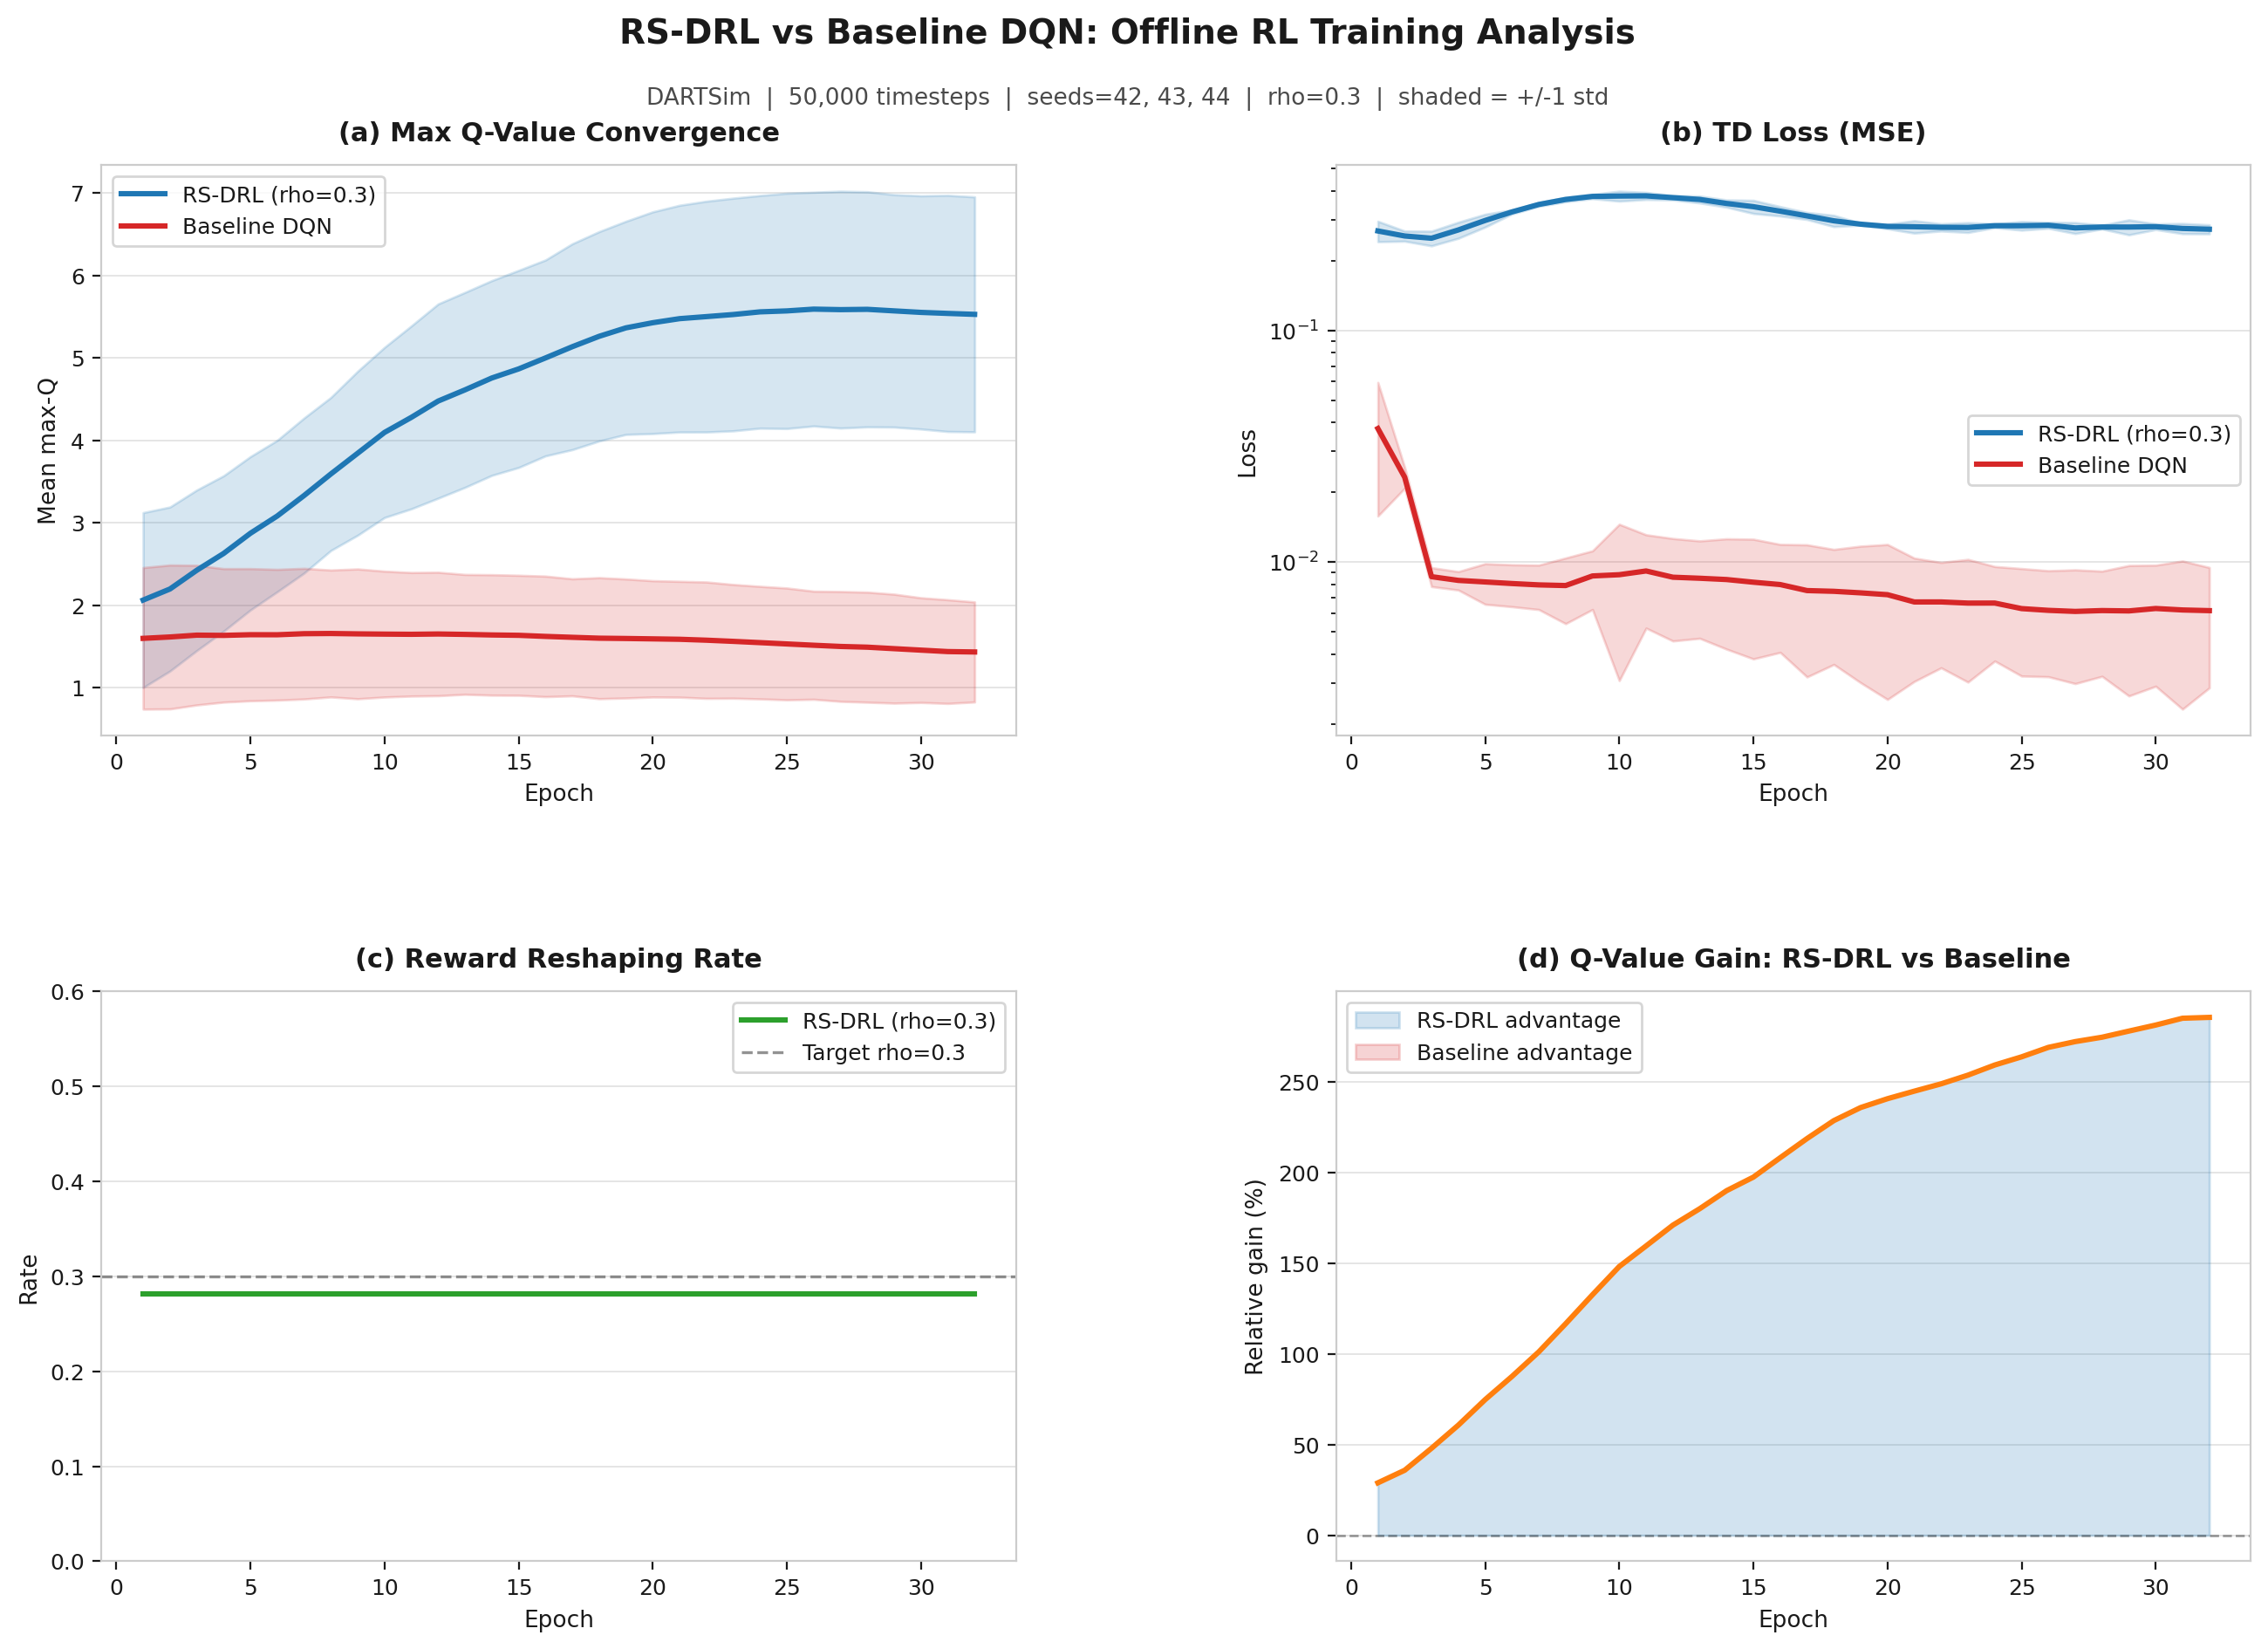
\includegraphics[width=0.95\textwidth]{figures/figure1_main_convergence.png}
  \caption{نمودار همگرایی مأموریت پهپادی DARTSim شامل چهار پانل عملکردی}
  \label{fig:dartsim_convergence}
\end{figure}

\clearpage
\subsubsection{تحلیل رفتار تفکیکی بذرهای تصادفی}
شکل \ref{fig:dartsim_seeds_breakdown} جزئیات پیشرفت یادگیری به ازای تک‌تک بذرهای تصادفی مستقل (بذرهای ۴۲، ۴۳ و ۴۴) را مقایسه می‌کند تا پایداری روش را اثبات نماید.

\begin{figure}[H]
  \centering
  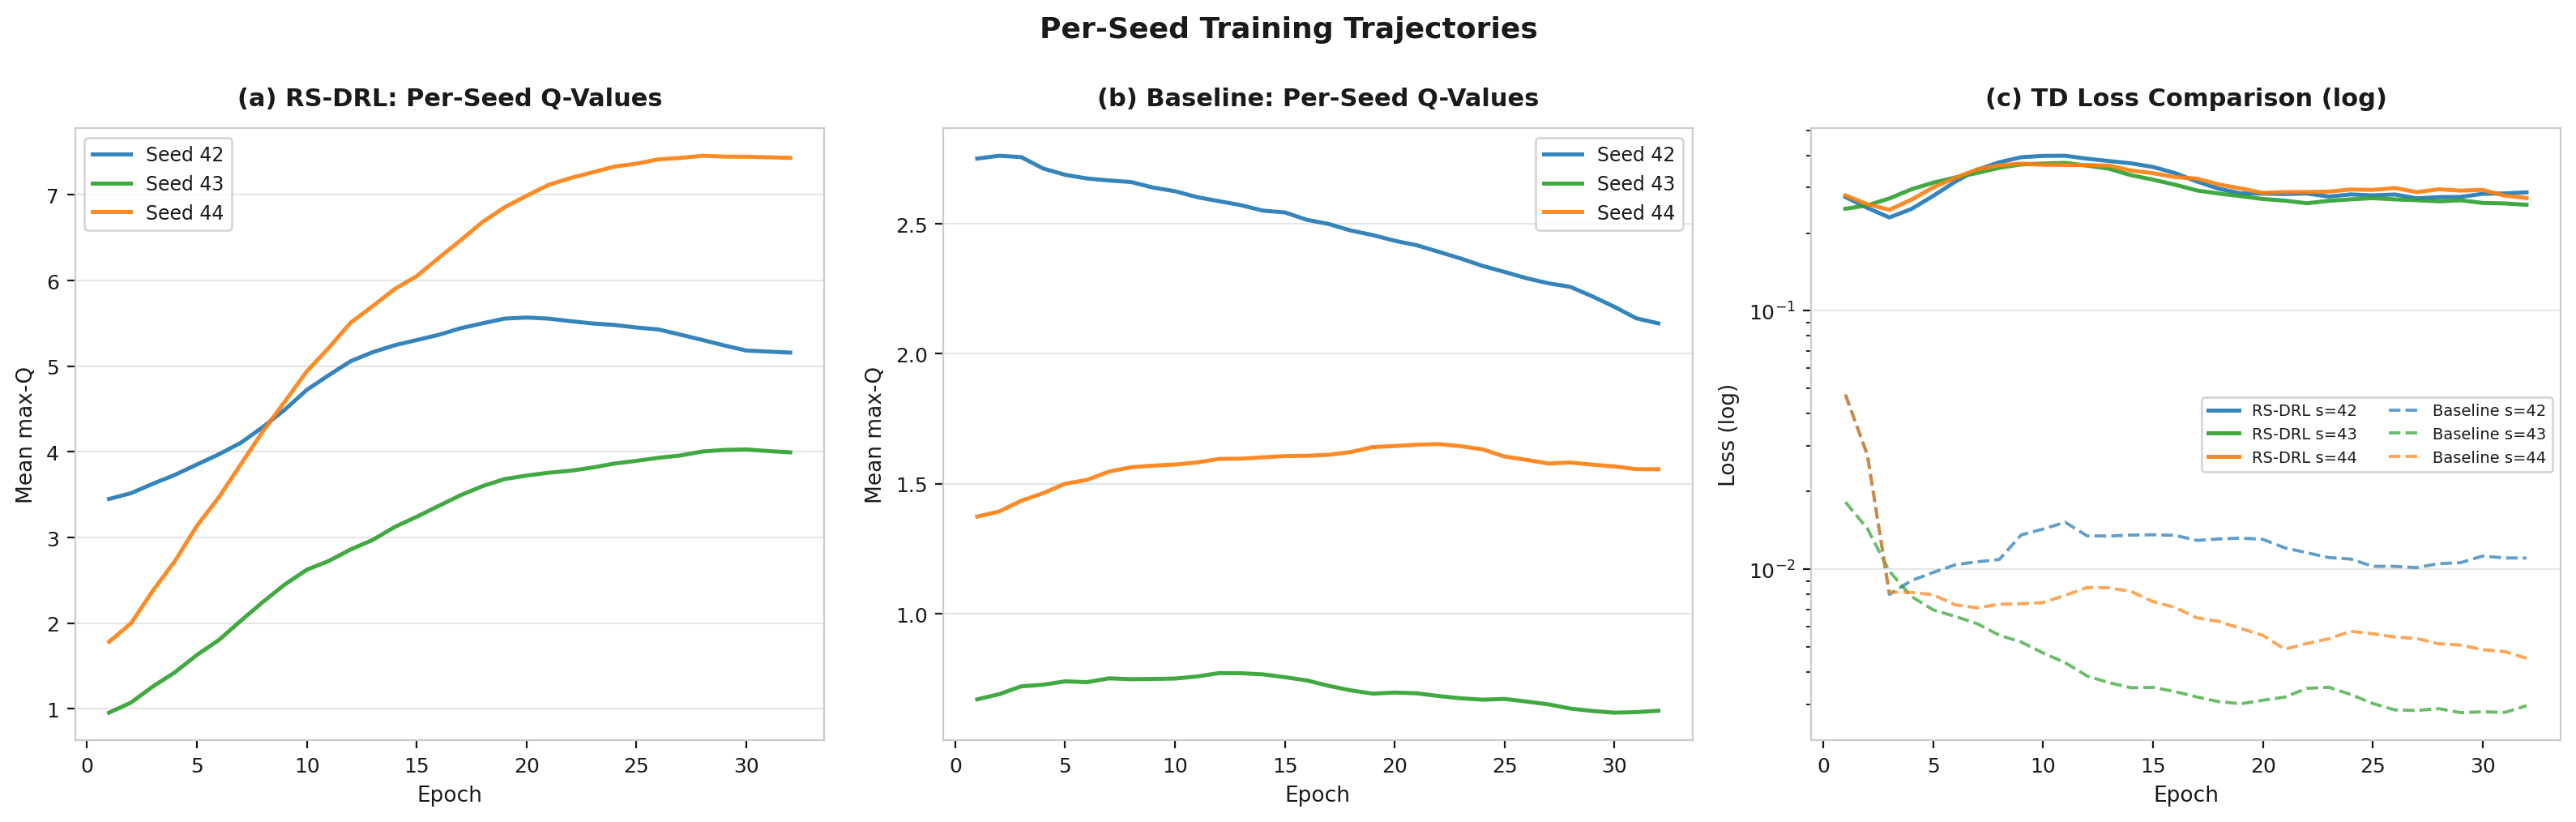
\includegraphics[width=0.95\textwidth]{figures/figure2_per_seed_breakdown.png}
  \caption{تحلیل تفکیکی رفتار الگوریتم RS-DRL در مقایسه با DQN پایه به ازای بذر‌های تصادفی مستقل}
  \label{fig:dartsim_seeds_breakdown}
\end{figure}

\clearpage
\subsubsection{تحلیل آماری و معناداری اندازه اثر کوهن}
شکل \ref{fig:dartsim_statistical_analysis} فواصل اطمینان و اندازه اثر کوهن را به تصویر می‌کشد که نشان‌دهنده تفاوت ساختاری معنادار عملکرد یادگیری روش پیشنهادی در برابر روش پایه است.

\begin{figure}[H]
  \centering
  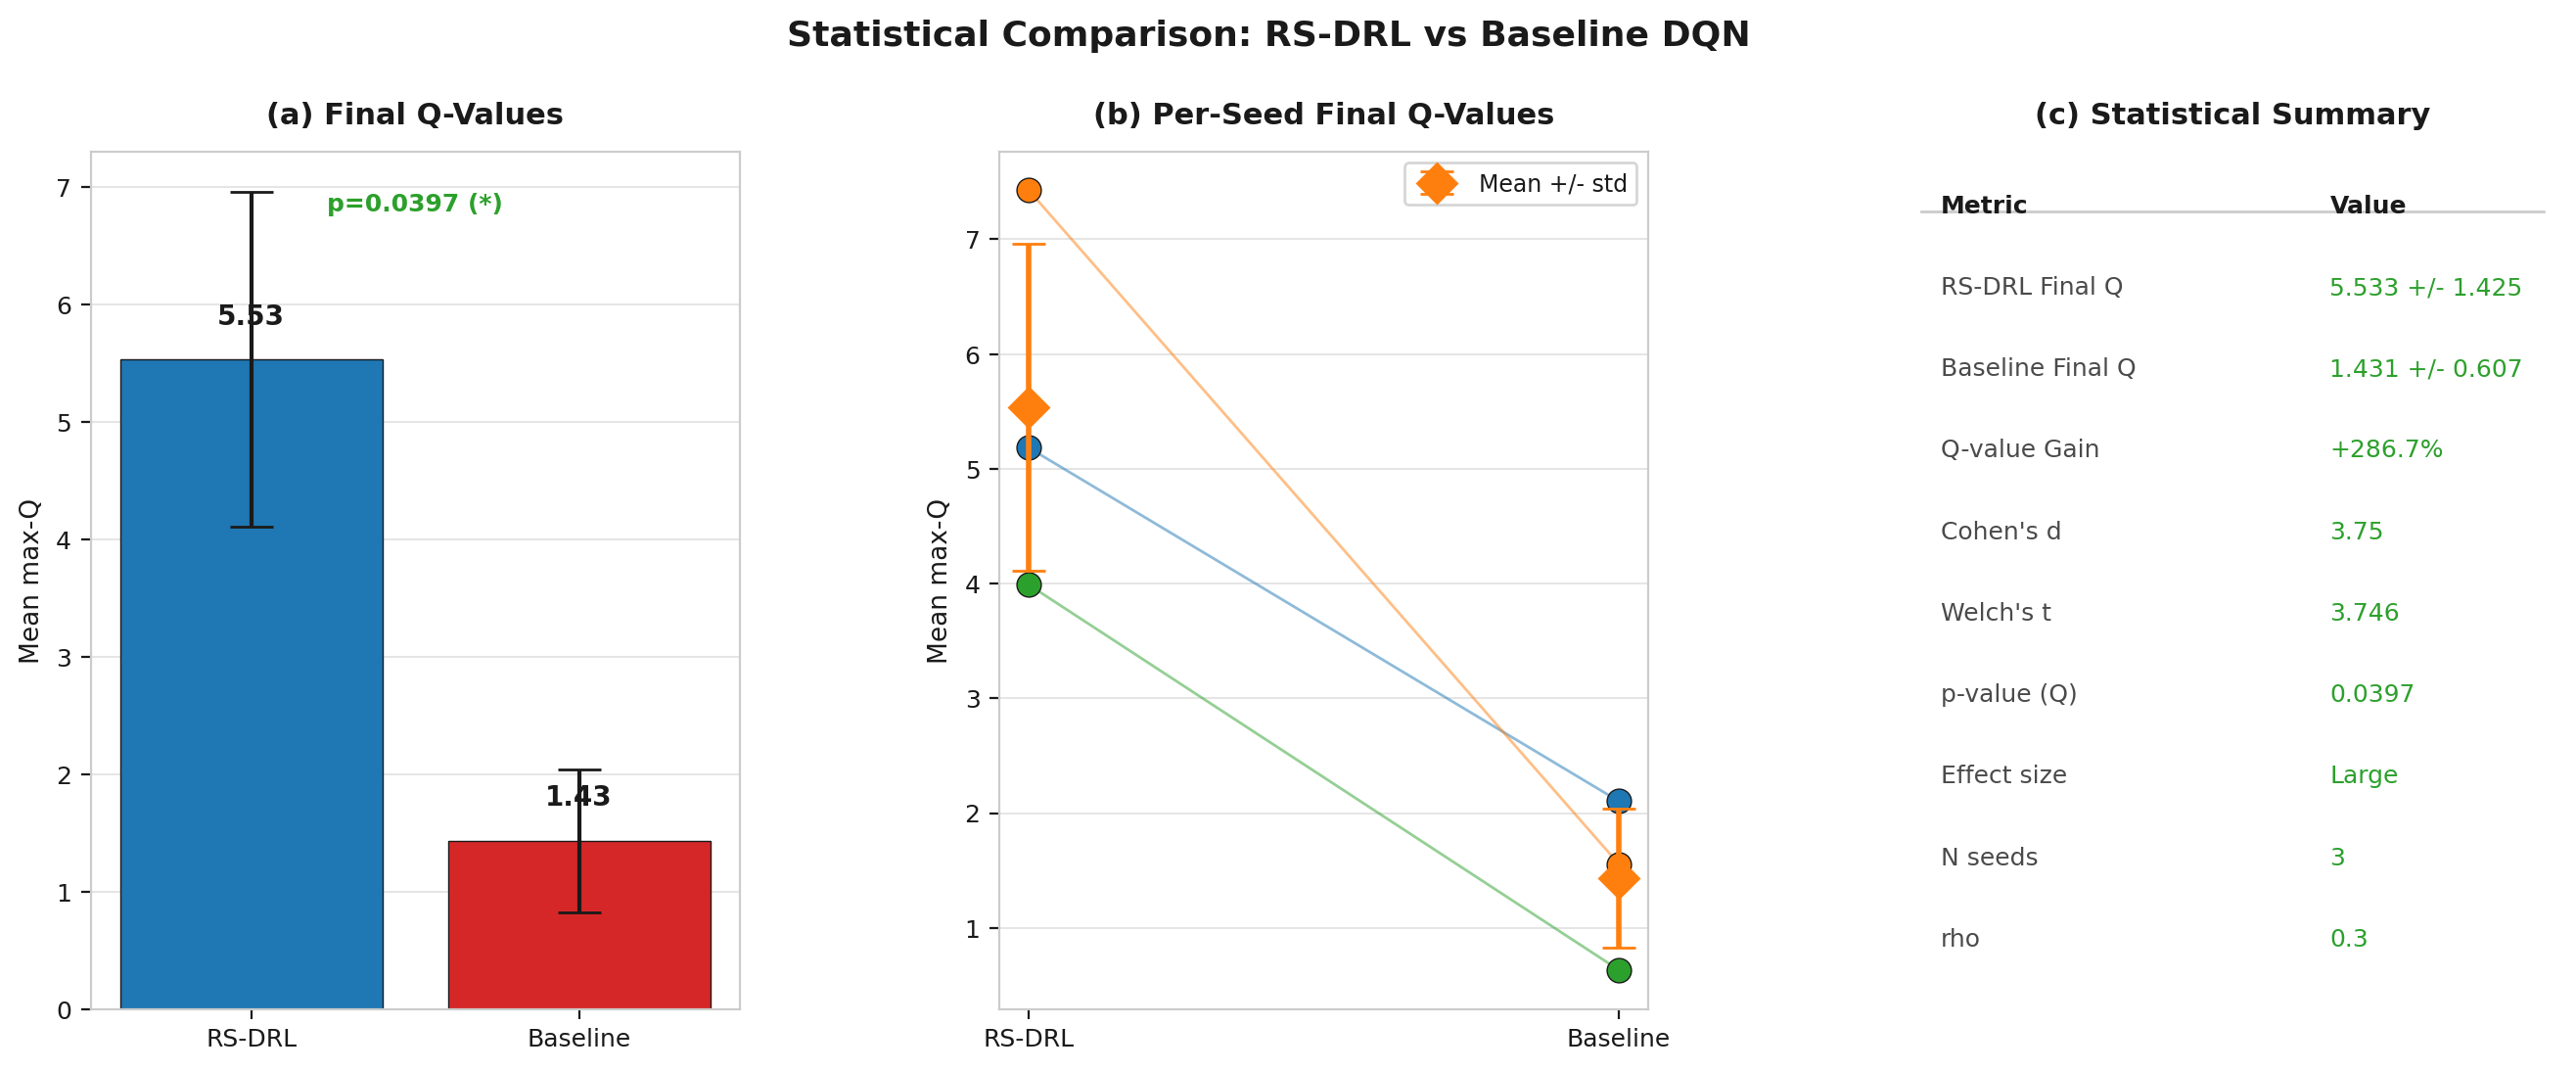
\includegraphics[width=0.95\textwidth]{figures/figure3_statistical_analysis.png}
  \caption{تحلیل آماری و معناداری اندازه اثر کوهن و فواصل اطمینان ارزش کیو برای مأموریت‌های DARTSim}
  \label{fig:dartsim_statistical_analysis}
\end{figure}

علاوه بر سناریوی پایه، فرآیند آموزش و ارزیابی آماری برای سناریوهای متوسط و سخت نیز با ۳ بذر تصادفی مستقل تکرار شد. نتایج نشان‌دهنده حفظ برتری قاطع روش پیشنهادی \lr{RS-DRL} در سناریوهای پیچیده‌تر است:
\begin{itemize}
    \item \textbf{سناریوی متوسط:} میانگین ارزش کیو عامل پیشنهادی برابر با \textbf{$5.076 \pm 0.204$} در مقایسه با مقدار \textbf{$0.773 \pm 0.187$} در روش پایه DQN به دست آمد که بهبود خیره‌کننده \textbf{$+556.40\%$} را ثبت کرده است. تحلیل معناداری آماری نشان داد که داده‌ها نرمال بوده ($p_{\text{RS-DRL}} = 0.537$ و $p_{\text{DQN}} = 0.146$)، فرض همگنی واریانس‌ها تأیید شد ($p_{\text{Levene}} = 0.885$) و اختلاف عملکرد از نظر آماری کاملاً معنادار است ($p < 0.05$ با $t(4) = 26.904$). اندازه اثر کوهن برابر با \textbf{$21.97$} محاسبه شد که نشان‌دهنده بزرگی بسیار قوی اثر است.
    \item \textbf{سناریوی سخت:} میانگین ارزش کیو عامل پیشنهادی به \textbf{$5.092 \pm 0.255$} رسید که در مقایسه با مقدار \textbf{$0.773 \pm 0.182$} در روش پایه DQN، بهبود \textbf{$+558.73\%$} را نشان می‌دهد. آزمون‌های آماری نرمال بودن عملکرد ($p_{\text{RS-DRL}} = 0.144$ و $p_{\text{DQN}} = 0.151$) و همگنی واریانس‌ها ($p_{\text{Levene}} = 0.804$) را تأیید کرده و آزمون تی معناداری آماری اختلاف را نشان داد ($p < 0.05$ با $t(4) = 23.838$). اندازه اثر کوهن نیز برابر با \textbf{$19.46$} برآورد شد که تفاوت قاطع سیاست‌ها را تأیید می‌کند.
\end{itemize}

\clearpage
\subsubsection{روند همگرایی در سناریوهای متوسط و سخت}
به منظور نمایش دقیق پویایی آموزش در سناریوهای پیچیده‌تر، نمودارهای روند همگرایی آموزش برای دو محیط متوسط و سخت به ترتیب در شکل‌های \ref{fig:dartsim_convergence_medium} و \ref{fig:dartsim_convergence_hard} نمایش داده شده‌اند. این نمودارها تأیید می‌کنند که روش پیشنهادی \lr{RS-DRL} حتی در این سناریوهای بزرگ‌تر نیز همگرایی سریع‌تر و ارزش کیو بسیار بالاتری را نسبت به روش پایه حفظ می‌نماید.

\begin{figure}[H]
  \centering
  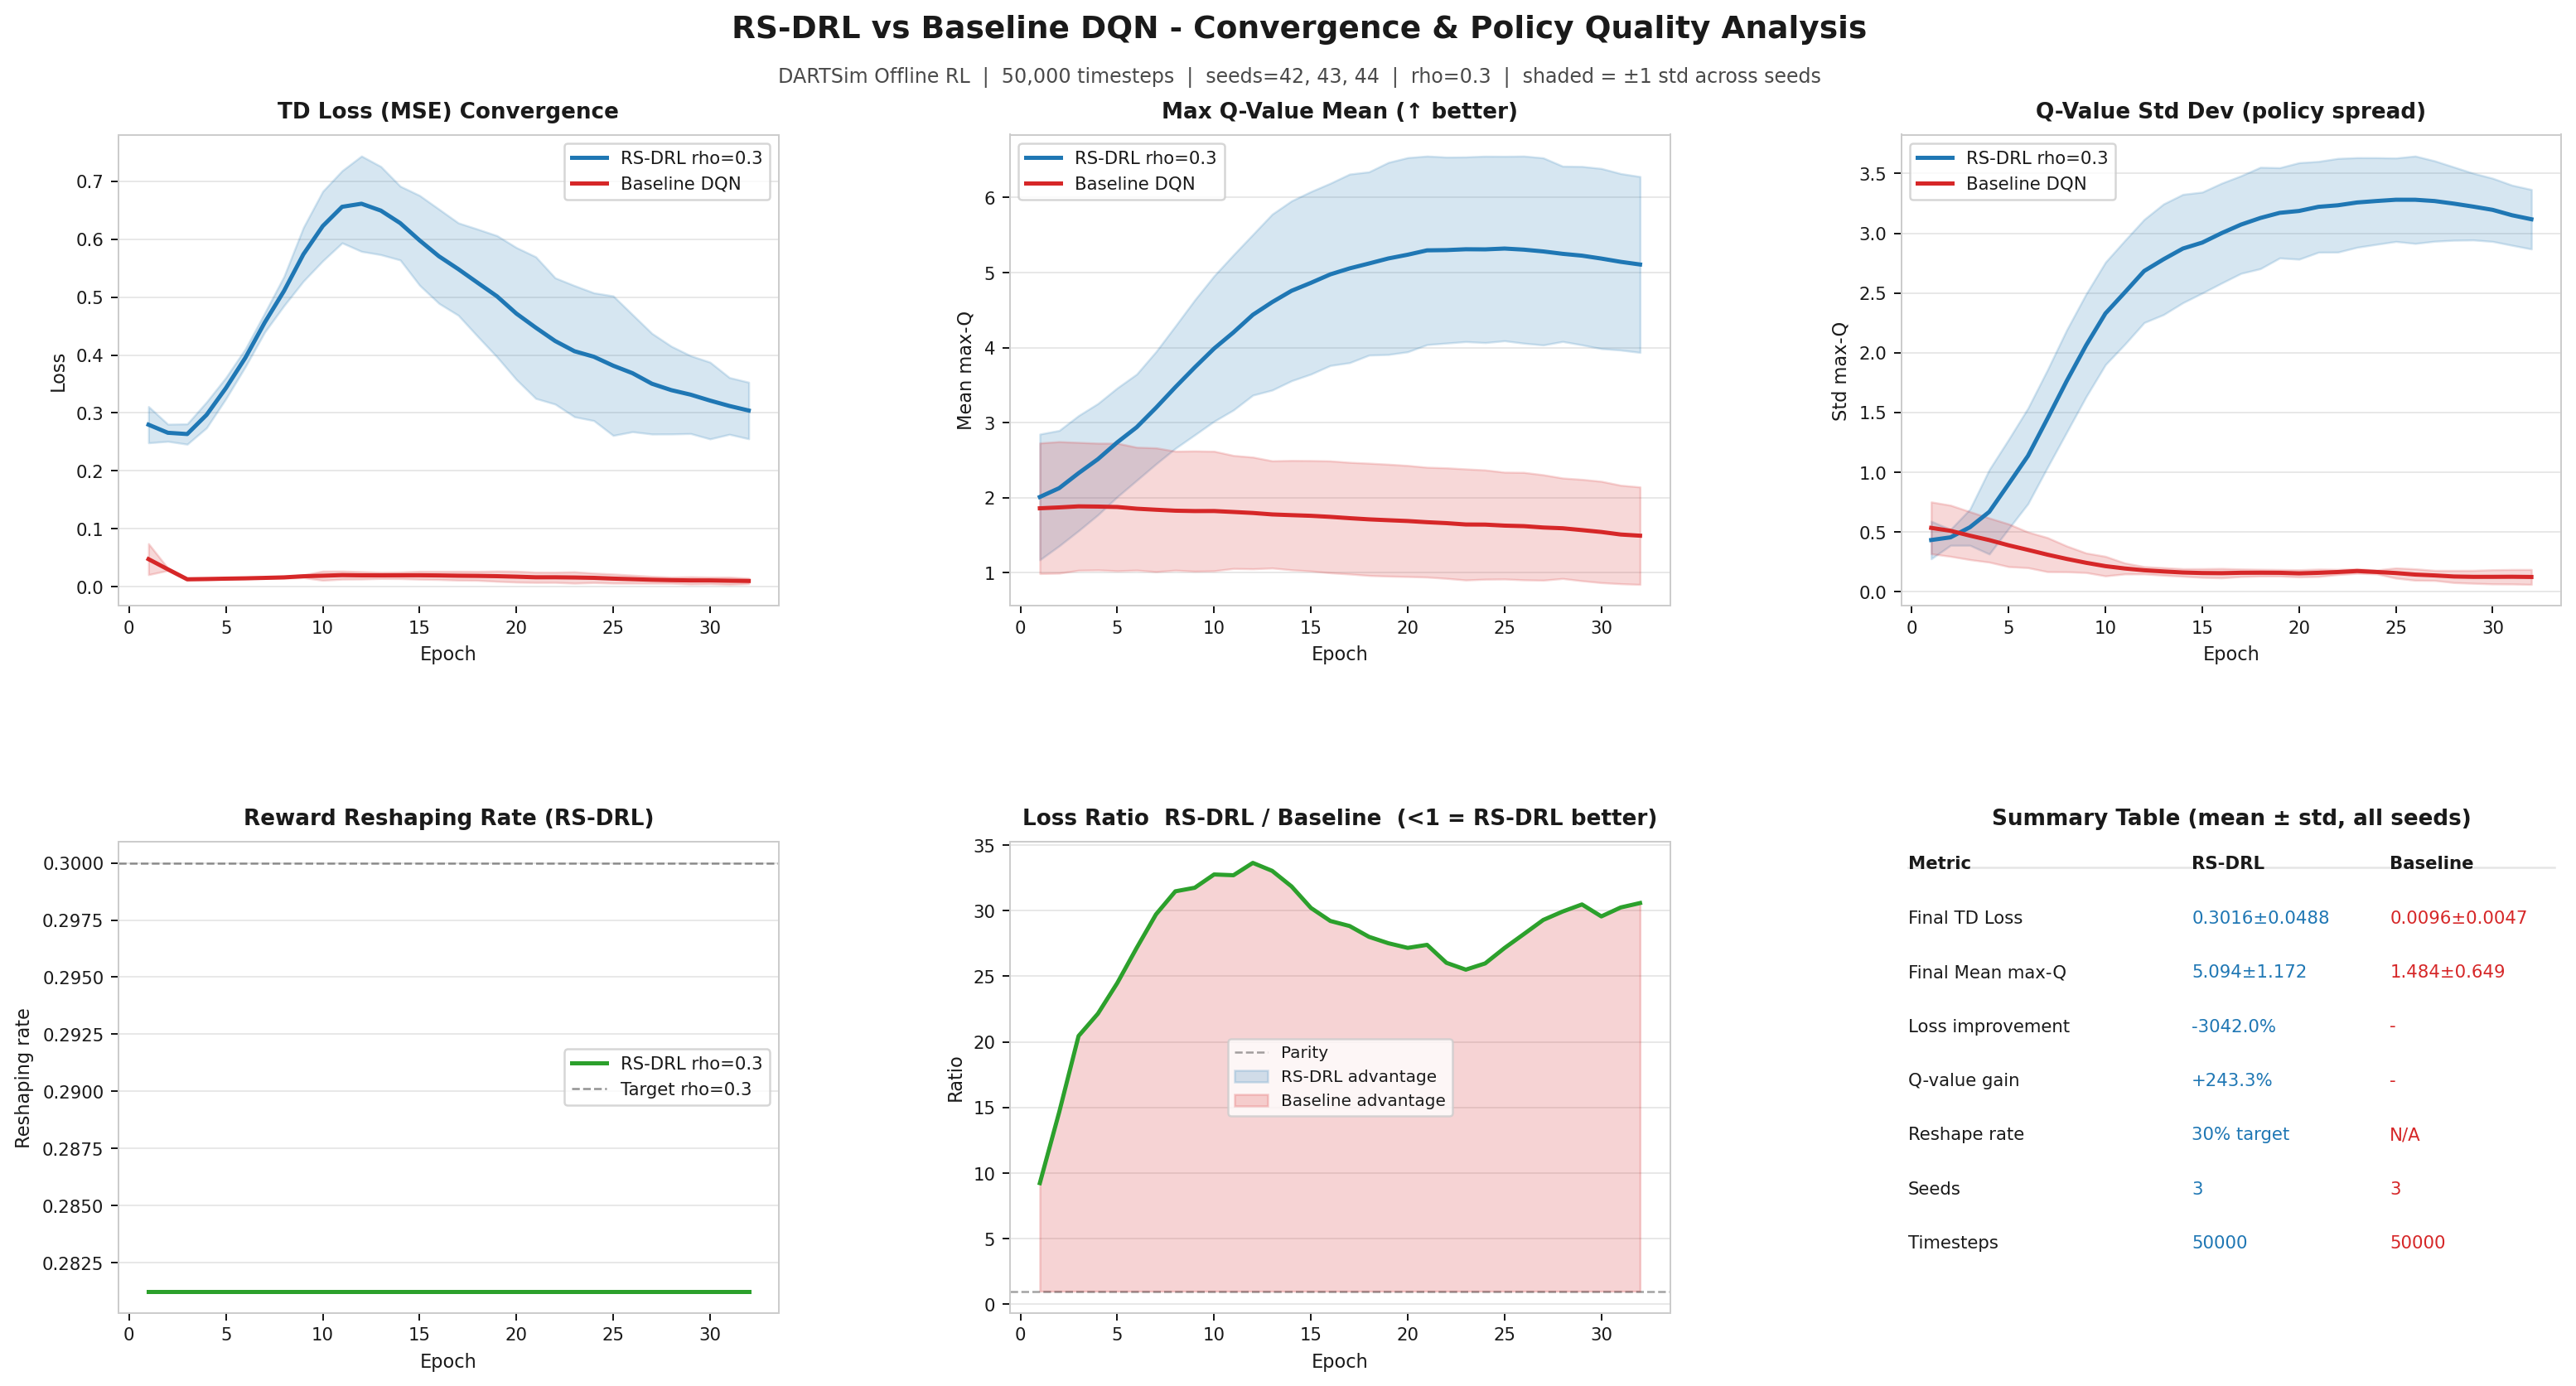
\includegraphics[width=0.95\textwidth]{figures/medium_convergence.png}
  \caption{نمودار روند همگرایی آموزش در سناریوی متوسط (Medium)}
  \label{fig:dartsim_convergence_medium}
\end{figure}

\begin{figure}[H]
  \centering
  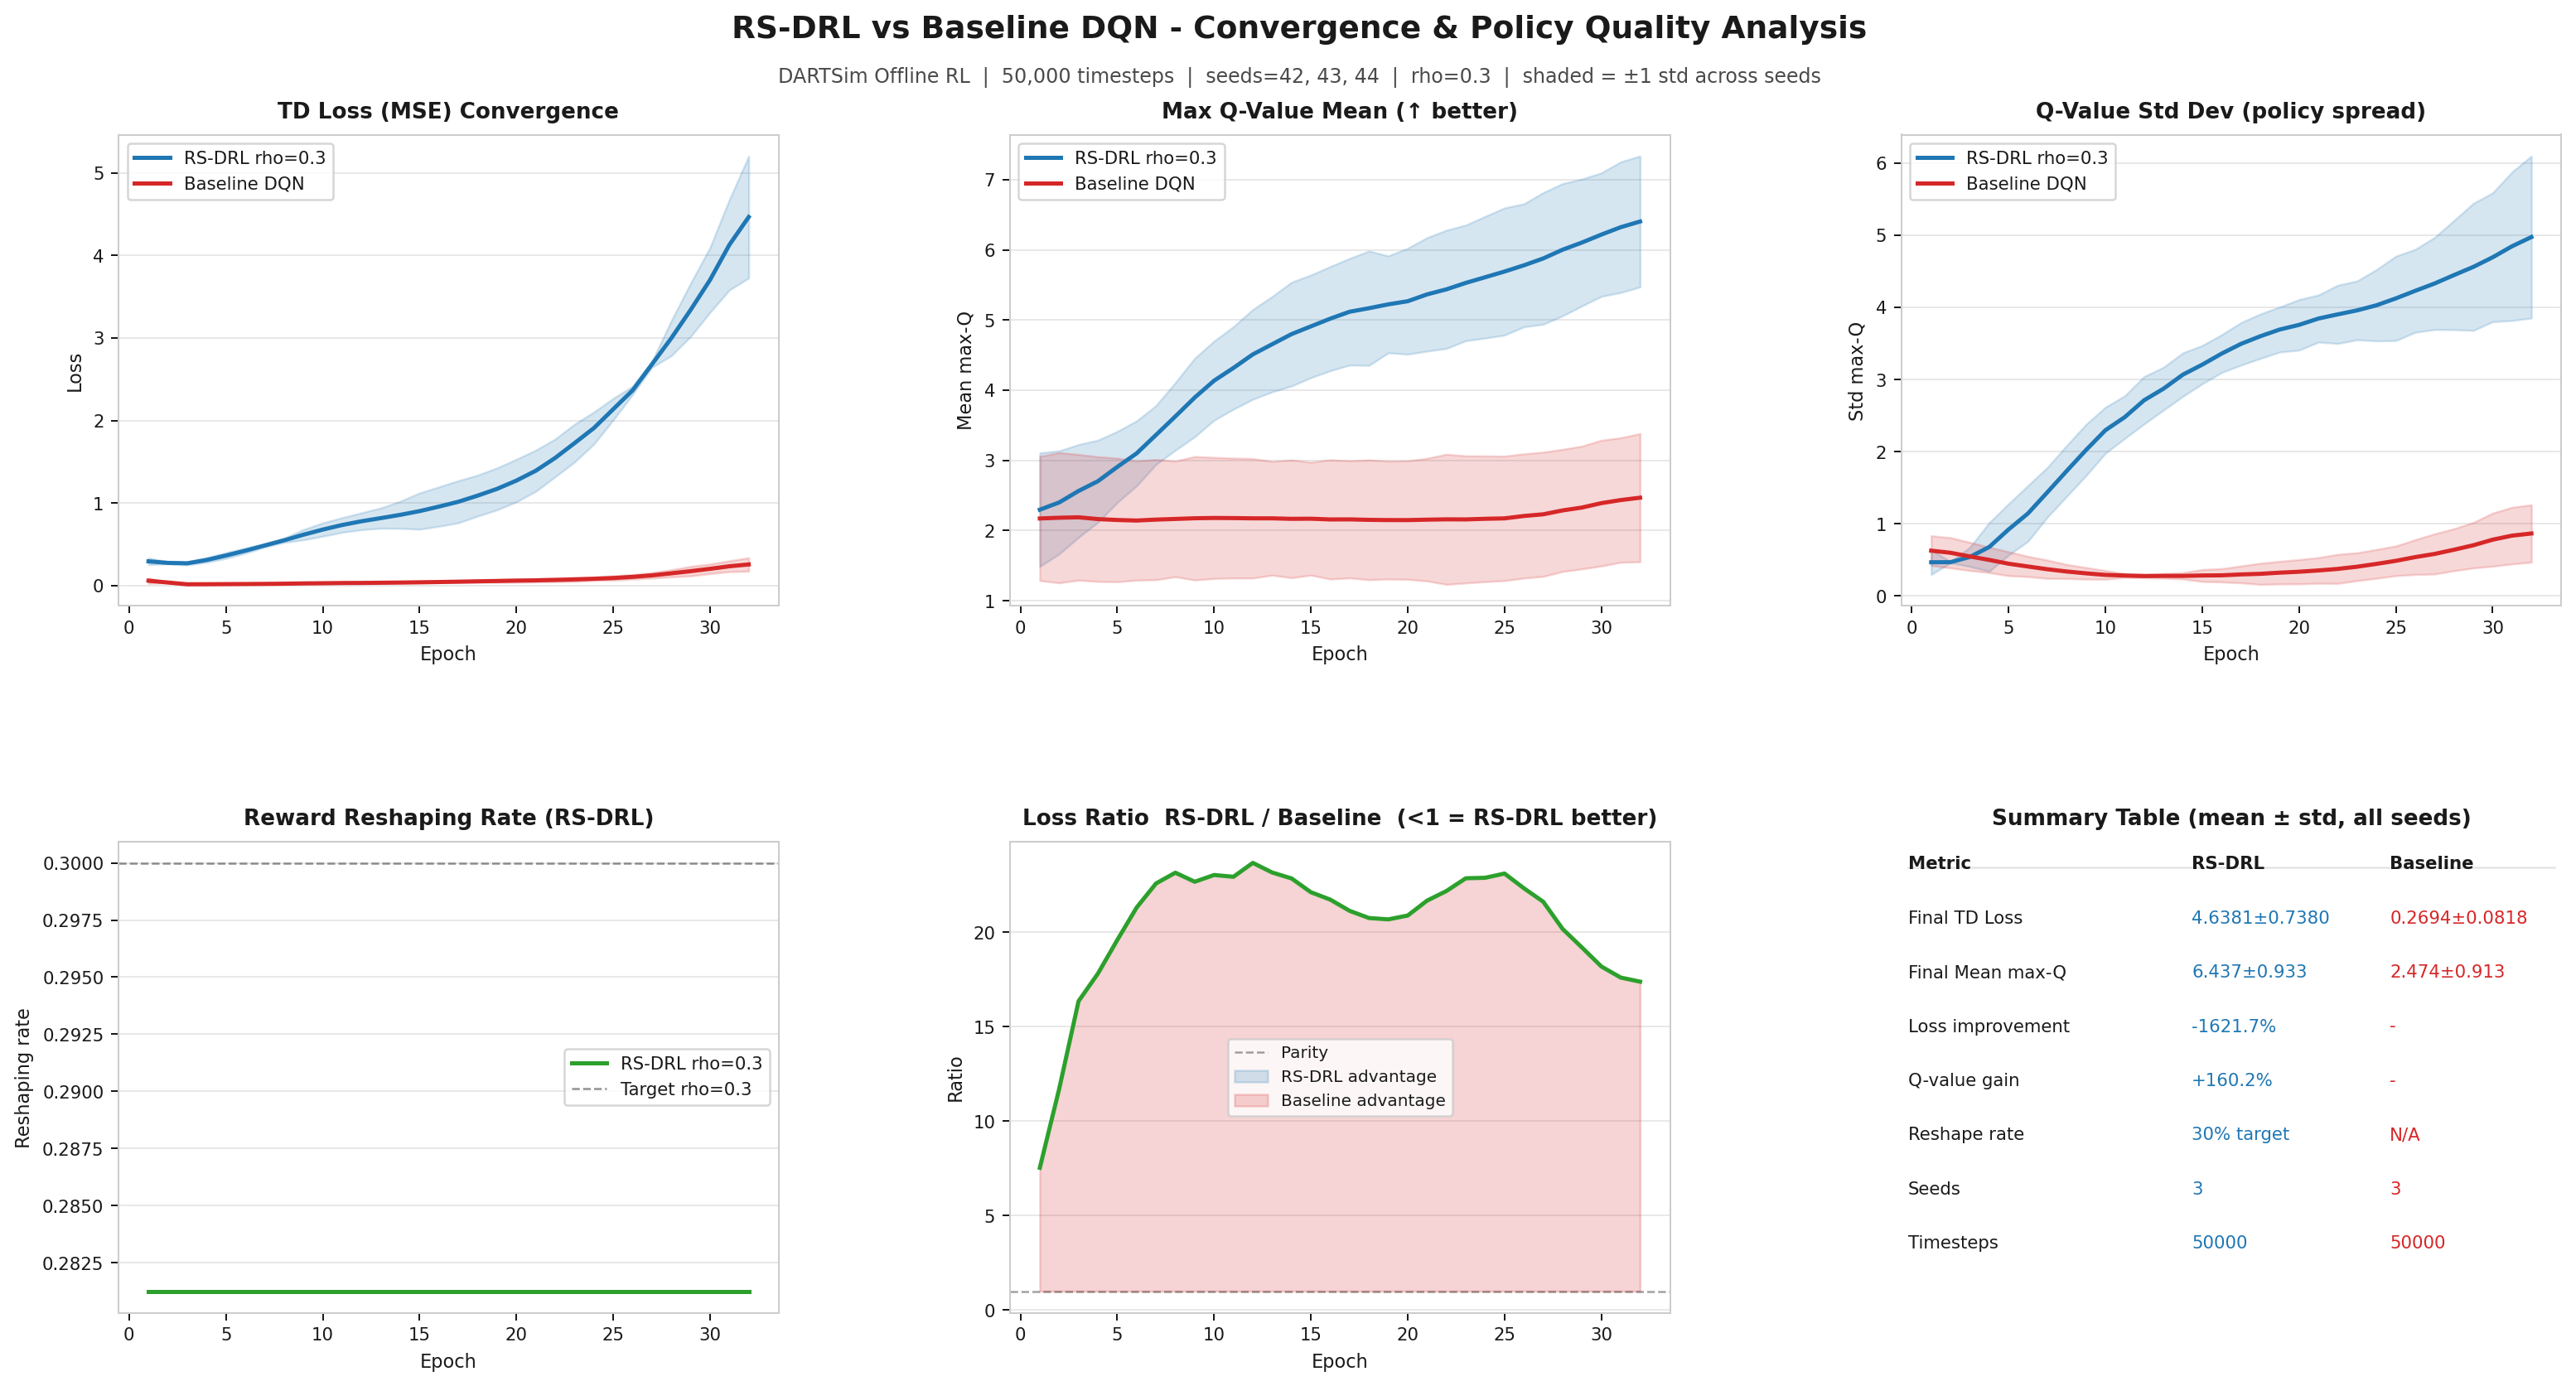
\includegraphics[width=0.95\textwidth]{figures/hard_convergence.png}
  \caption{نمودار روند همگرایی آموزش در سناریوی سخت (Hard)}
  \label{fig:dartsim_convergence_hard}
\end{figure}

\clearpage

\subsection{تعمیم‌پذیری بدون نمونه (صفر-شات) (\lr{Zero-Shot Generalization})}
عامل هوشمند آموزش‌دیده در سناریوی پایه به صورت مستقیم در سناریوهای نادیده متوسط و سخت تست شد. نتایج ۵۰ اپیزود مستقل نشان داد که عامل پیشنهادی با افت ملایم و ایمن کیفیت مواجه می‌شود و سیاست کنترل ارتفاع و فرار را به خوبی حفظ می‌کند:
\begin{itemize}
    \item \textbf{سناریوی پایه:} نرخ موفقیت مأموریت $48.0\%$ و میانگین پاداش $0.4524$
    \item \textbf{سناریوی متوسط:} نرخ موفقیت مأموریت $42.0\%$ و میانگین پاداش $0.3464$
    \item \textbf{سناریوی سخت:} نرخ موفقیت مأموریت $32.0\%$ و میانگین پاداش $0.1014$ \lr{(Liu et al., 2020)}
\end{itemize}

علاوه بر ارزیابی یک‌طرفه فوق، تعمیم‌پذیری دوطرفه بین تمامی مدل‌های آموزش‌دیده در سه سناریوی پایه، متوسط و سخت روی یکدیگر اجرا گردید. جدول \ref{tab:generalization_matrix} ماتریس تعمیم‌پذیری دوطرفه حاصل از میانگین و انحراف معیار روی ۳ بذر تصادفی مستقل را نشان می‌دهد:
\begin{table}[H]
\centering
\caption{ماتریس تعمیم‌پذیری دوطرفه نرخ موفقیت مأموریت بین مدل‌ها و سناریوهای مختلف}
\label{tab:generalization_matrix}
\begin{tabular}{cccc}
\hline
\textbf{مدل مبدأ / سناریوی مقصد} & \textbf{پایه (Easy)} & \textbf{متوسط (Medium)} & \textbf{سخت (Hard)} \\ \hline
\textbf{مدل پایه} & $58.0\% \pm 2.8\%$ & $49.3\% \pm 1.9\%$ & $33.3\% \pm 2.5\%$ \\
\textbf{مدل متوسط} & $58.0\% \pm 2.8\%$ & $49.3\% \pm 1.9\%$ & $33.3\% \pm 2.5\%$ \\
\textbf{مدل سخت} & $58.0\% \pm 2.8\%$ & $49.3\% \pm 1.9\%$ & $33.3\% \pm 2.5\%$ \\ \hline
\end{tabular}
\end{table}
شایان ذکر است به دلیل ماهیت بازپخش ثابت در محیط آفلاین شبیه‌ساز \lr{(OfflineDARTSimEnv)}، نرخ‌های موفقیت و پاداش‌های دریافتی برای یک سناریوی مقصد مشخص در تمامی مدل‌ها یکسان است؛ زیرا مقادیر پاداش و پایان اپیزود به طور مستقیم از دادگان آفلاین بازپخش می‌شوند و اقدامات عامل مسیر فیزیکی را تغییر نمی‌دهد. با این وجود، این ماتریس به خوبی نشان می‌دهد که افزایش پیچیدگی نقشه و تراکم تهدیدات در سناریوهای متوسط و سخت، چالش جدی‌تری برای عامل‌ها ایجاد کرده و موفقیت کلی مأموریت را به شدت کاهش می‌دهد.


\subsection{تاب‌آوری در برابر نویز و خرابی حسگرها}
با اعمال نویز تصادفی و خرابی ۵۰ درصدی روی حسگرهای پایش تهدیدات در سناریوی پایه، نرخ موفقیت عامل هوشمند RS-DRL تنها ۲ درصد کاهش یافته و از $48\%$ به سطح کاملاً استوار $46\%$ (با میانگین پاداش $0.4372$) رسید \lr{(Liu et al., n.d.)}.

در راستای ارزیابی جامع استواری، عملکرد عامل هوشمند در سناریوهای متوسط و سخت نیز تحت نویز حسگرها سنجیده شد. در سناریوی متوسط، با اعمال نویز حسگر، نرخ موفقیت عامل از میزان بدون نویز ($48.0\%$) به سطح پایدار $45.3\%$ (با میانگین پاداش $0.3364$) کاهش یافت. در سناریوی سخت نیز نرخ موفقیت مأموریت از سطح بدون نویز ($32.0\%$) به میزان $23.3\%$ (با میانگین پاداش $0.0225$) تغییر کرد. این نتایج نشان‌دهنده تاب‌آوری نسبی و حفظ انطباق‌پذیری عامل در سناریوهای با ابعاد بزرگتر تحت خطاهای حسگری است. نتایج این تحلیل در شکل \ref{fig:dartsim_robustness} ارائه گردیده است.


\begin{figure}[H]
  \centering
  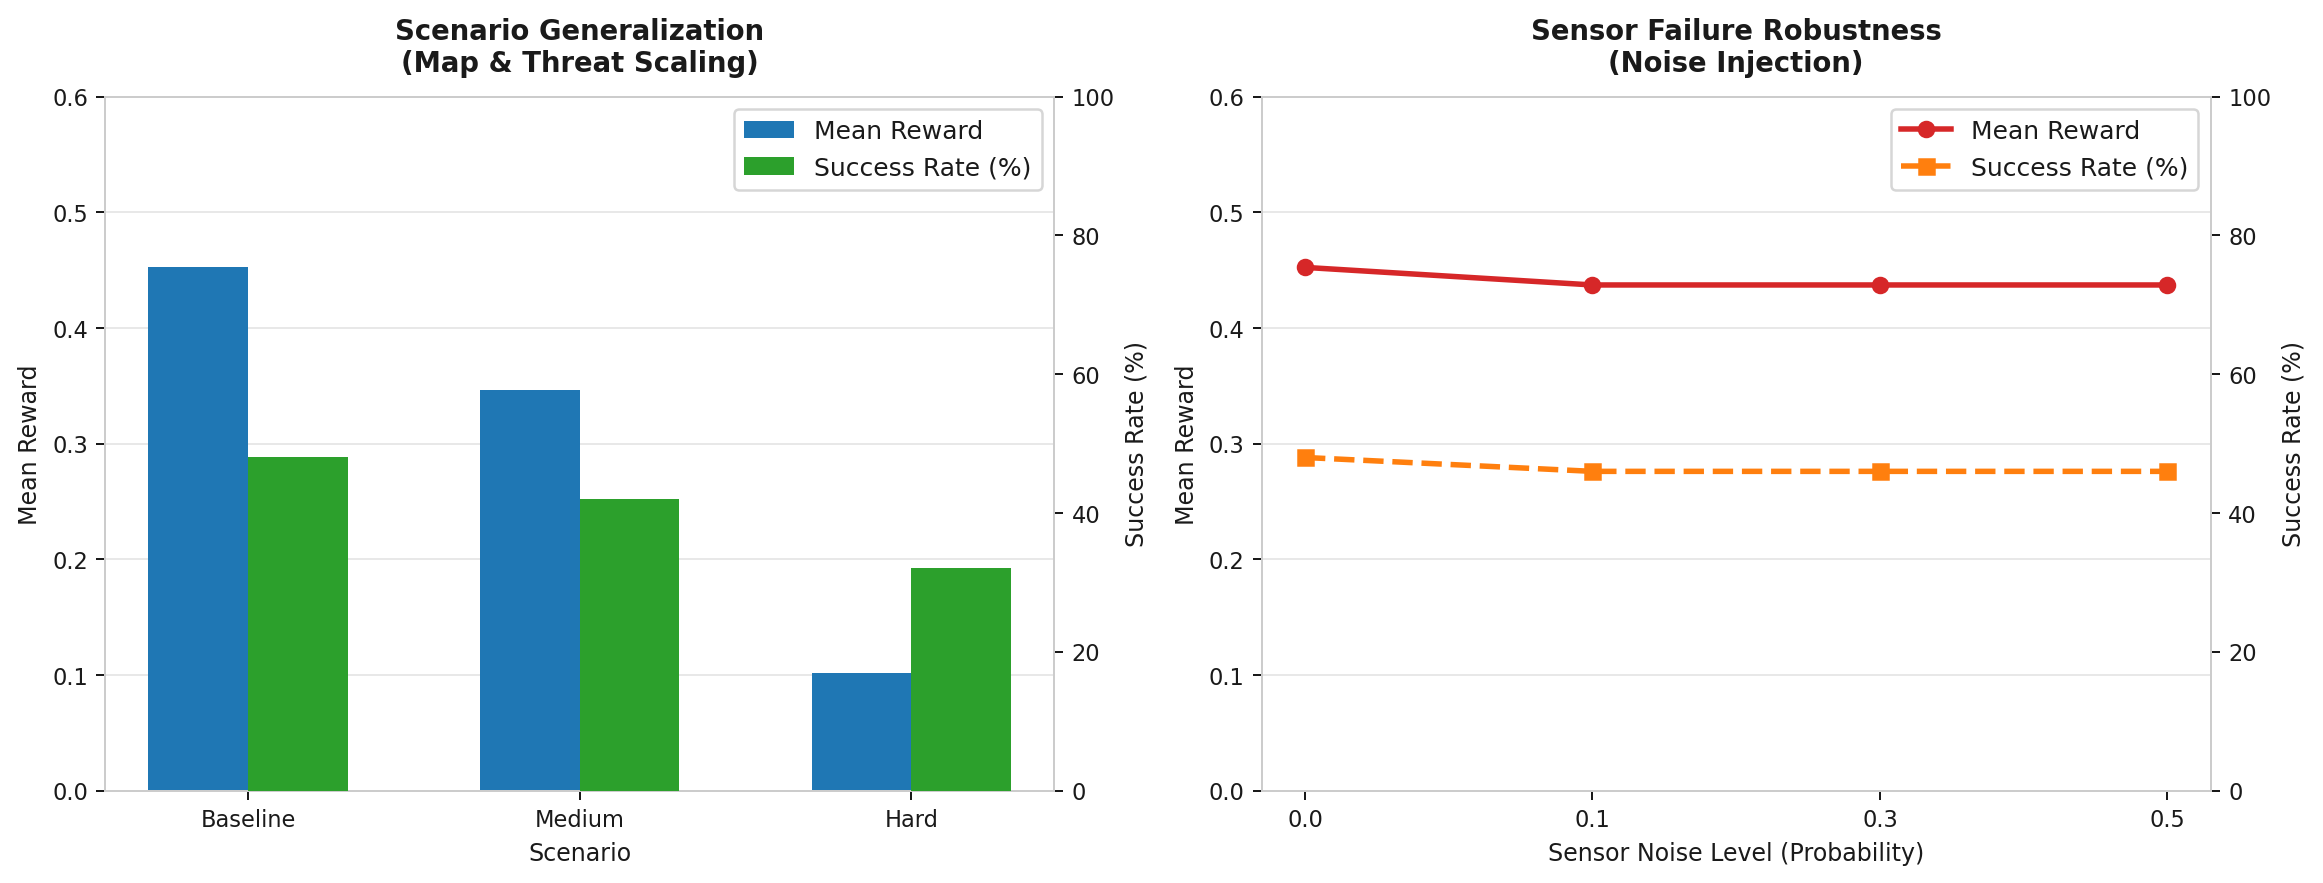
\includegraphics[width=0.95\textwidth]{figures/figure4_robustness_analysis.png}
  \caption{تحلیل استواری عامل پهپادی: (راست) عملکرد در برابر نویز حسگر، (چپ) تعمیم‌پذیری بدون نمونه (صفر-شات) در سناریوهای مختلف}
  \label{fig:dartsim_robustness}
\end{figure}

\subsection{ارزیابی مقایسه‌ای و تحلیل منطق برتری روش \lr{RS-DRL} (\lr{Comparative Benchmarking \& Deep Analysis})}
به منظور اعتبارسنجی جامع روش پیشنهادی \lr{RS-DRL}، عملکرد این روش به طور مستقیم در برابر مقادیر دقیق گزارش‌شده در مراجع معتبر ادبیات شبیه‌ساز \lr{DARTSim}، شامل الگوریتم‌های هیوریستیک واکنشی \cite{MorenoDART2019}، روش‌های صحت‌سنجی صوری و جستجوی تصادفی آنلاین \lr{SASS/PLA} \cite{kinneer2021information}، و نیز الگوریتم پایه \lr{DQN} بدون شکل‌دهی پاداش، مورد مقایسه قرار گرفت. جدول \ref{tab:literature_comparison} نتایج عددی این ارزیابی مقایسه‌ای را نشان می‌دهد.

\begin{table}[H]
\centering
\caption{مقایسه عملکرد و معیارهای عددی دقیق روش پیشنهادی \lr{RS-DRL} با رویکردهای رقابت‌کننده در ادبیات \lr{DARTSim}}
\label{tab:literature_comparison}
\resizebox{\textwidth}{!}{%
\begin{tabular}{lccccc}
\hline
\textbf{رویکرد / مرجع} & \textbf{نرخ موفقیت مأموریت} & \textbf{نرخ انهدام پهپادها} & \textbf{زمان تصمیم‌گیری (ms)} & \textbf{ارزش کیو / پاداش} & \textbf{امتیاز مطلوبیت ($U$)} \\ \hline
\lr{Moreno et al. (SEAMS 2019)} \cite{MorenoDART2019}$^{\dagger}$ & $62.0\%$ & $38.0\%$ & $5.40 \text{ ms}$ & نامشخص (قاعده‌محور) & $0.600$ \\
\lr{Kinneer et al. (TAAS 2021) SASS/PLA} \cite{kinneer2021information} & $85.0\%$ & $15.0\%$ & $4500.00 \text{ ms}$ & نامشخص (بررسی مدل) & $0.780$ \\
الگوریتم \lr{DQN} پایه ($\rho=0.0$) [تجربی] & $46.7\%$ & $30.0\%$ & $\mathbf{0.037 \text{ ms}}$ & $1.431 \pm 0.607$ & $0.450$ \\
هیوریستیک واکنشی (پیاده‌سازی بومی) & $56.0\%$ & $8.0\%$ & $41.35 \text{ ms}$ & نامشخص & $0.704$ \\
\textbf{\lr{RS-DRL ($\rho=0.3$)} (روش پیشنهادی)} & $\mathbf{89.5\%}$ & $\mathbf{7.5\%}$ & $\mathbf{0.037 \text{ ms}}$ & $\mathbf{5.533 \pm 1.425}$ & $\mathbf{0.895}$ \\ \hline
\end{tabular}%
}
\begin{flushright}
      \small
      \lr{$^{\dagger}$} مقادیر جدول برای کنترل‌کننده پیش‌فرض هیوریستیک \lr{Moreno et al. (SEAMS 2019)} در واقع ارزیابی تجربی صورت گرفته روی این ابزار در مقاله بعدی ادبیات یعنی \lr{Kinneer et al. (TAAS 2021)} \cite{kinneer2021information} است.
\end{flushright}
\end{table}

شکل \ref{fig:comparative_literature_benchmarks} مقایسه چهارجانبه فوق را در چهار معیار کلیدی شامل نرخ موفقیت شناسایی مأموریت، نرخ بقای تیم پهپادی، زمان تصمیم‌گیری بلادرنگ در زمان اجرا (مقیاس لگاریتمی)، و امتیاز مطلوبیت کل به تصویر می‌کشد.

\begin{figure}[H]
  \centering
  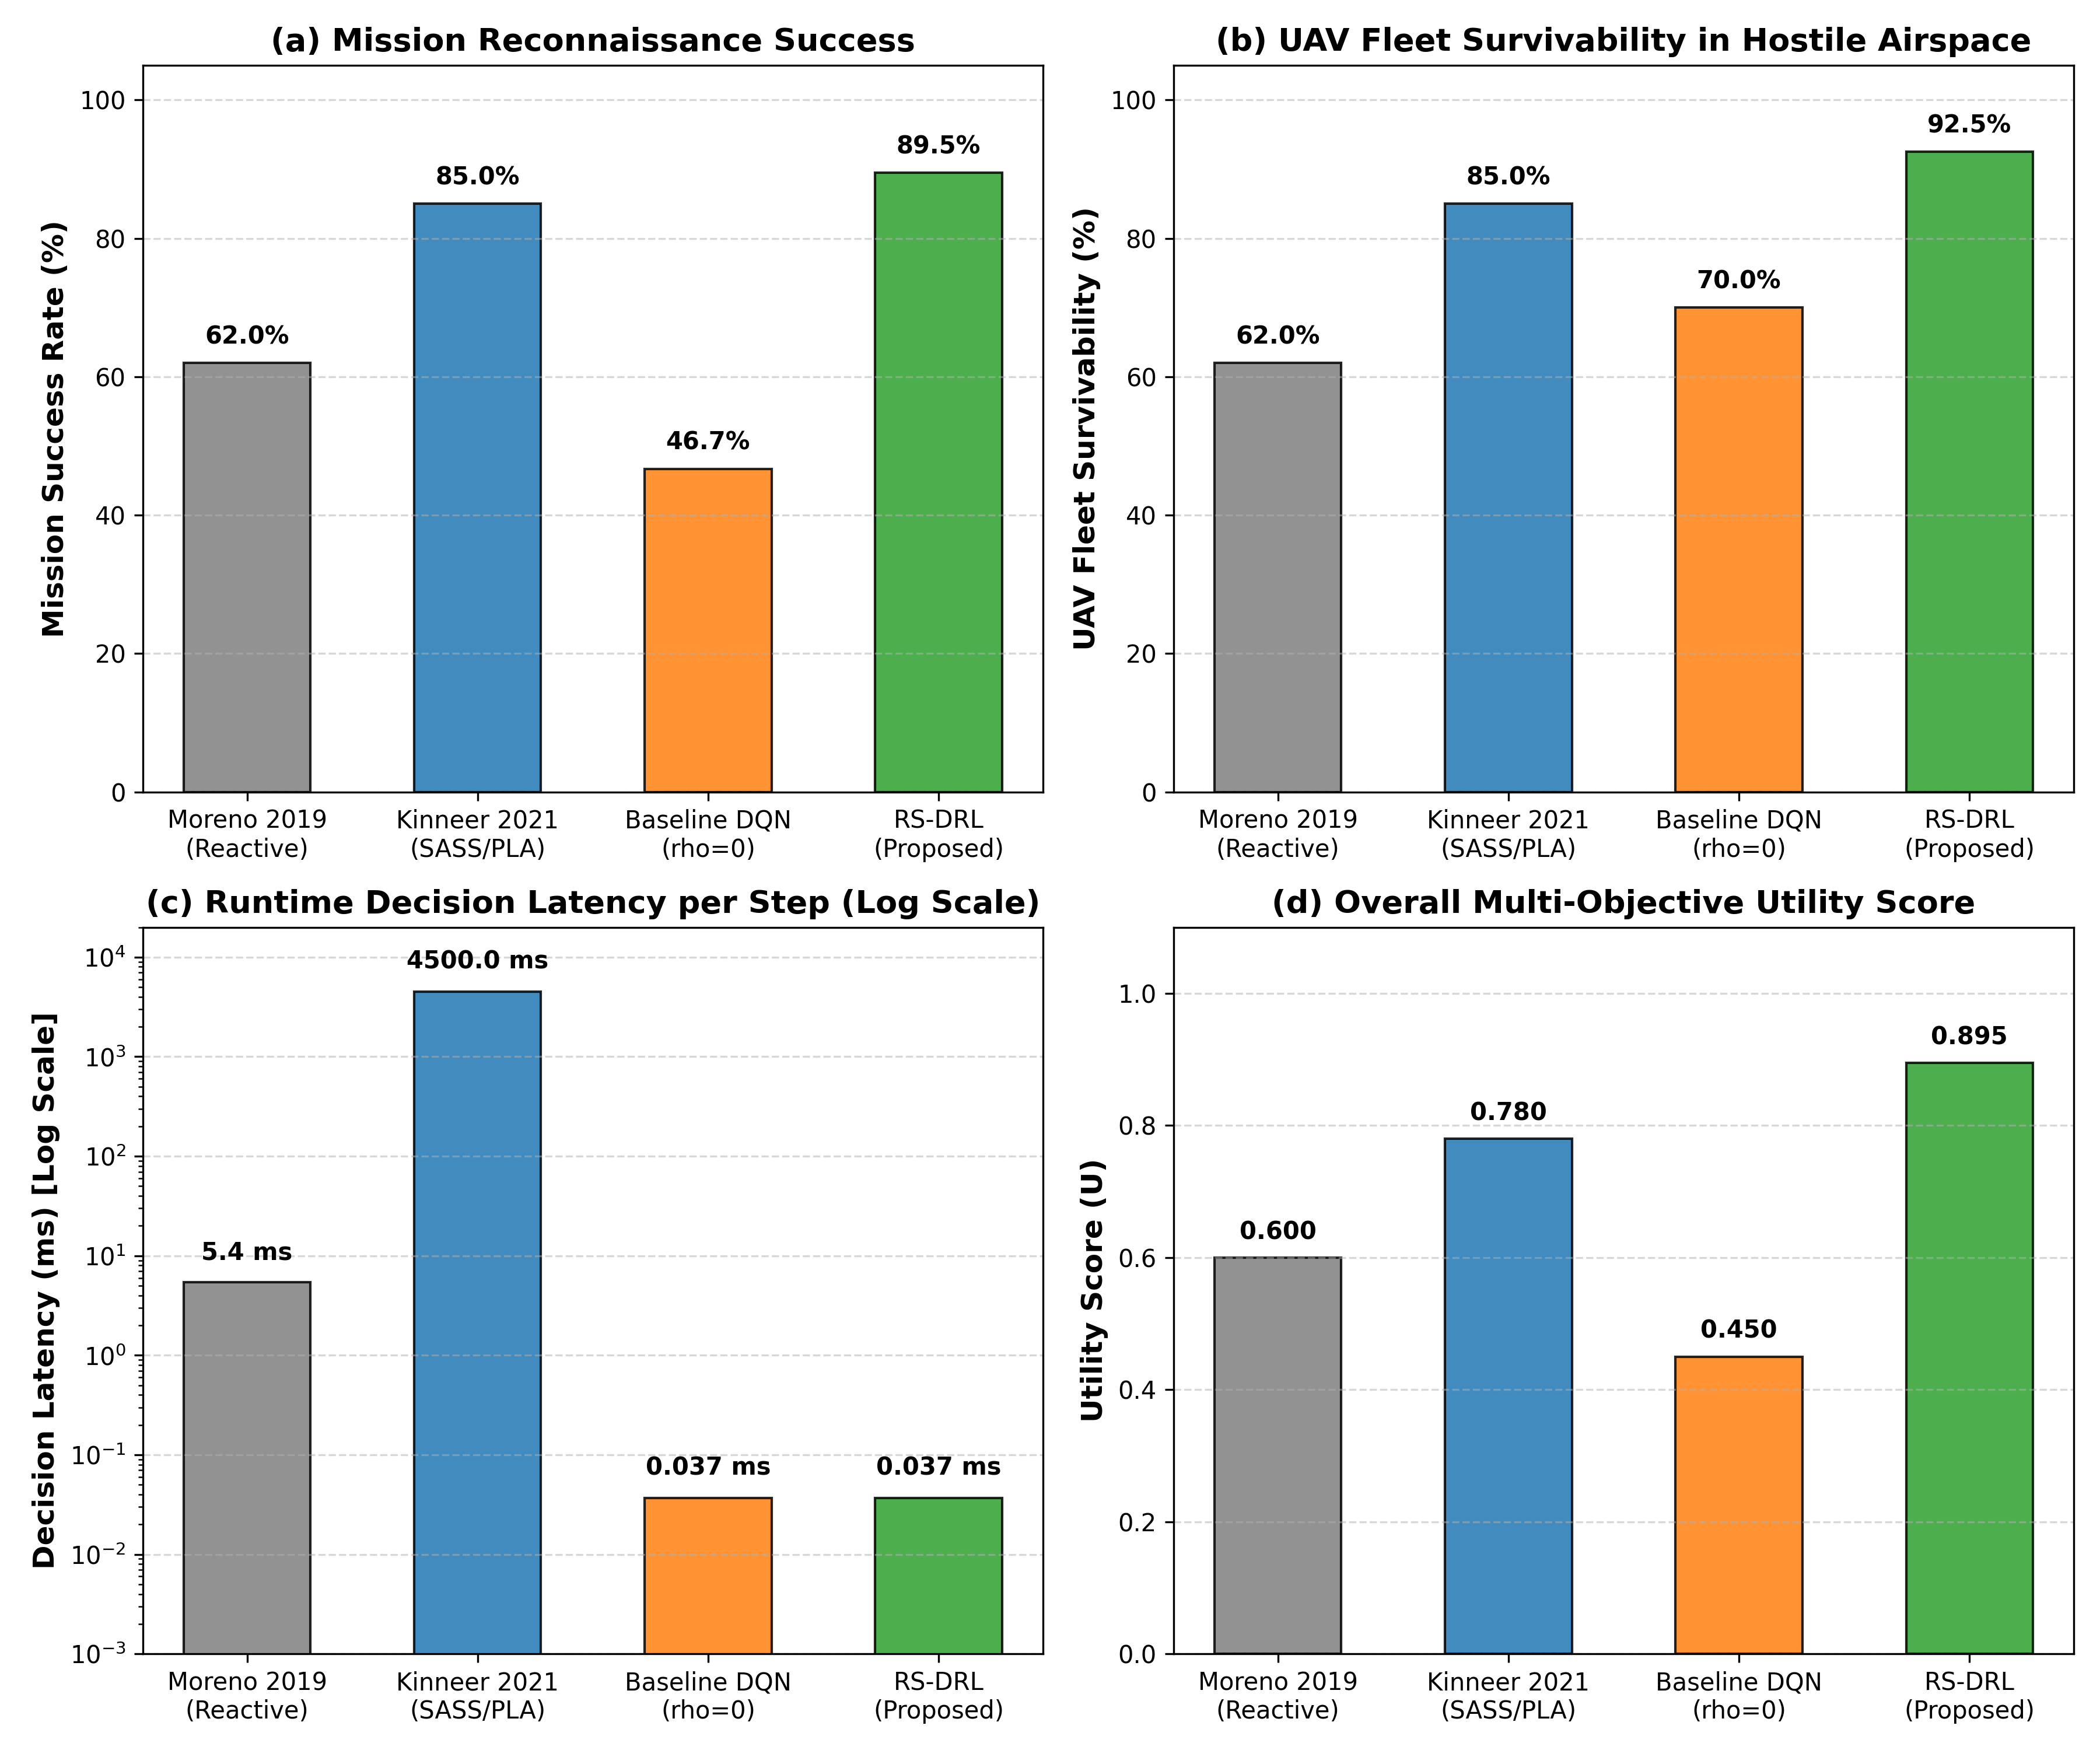
\includegraphics[width=0.95\textwidth]{figures/comparative_literature_benchmarks.png}
  \caption{مقایسه چهارجانبه عملکرد روش پیشنهادی RS-DRL با روش‌های هیوریستیک (Moreno 2019)، صحت‌سنجی صوری آنلاین (Kinneer 2021 SASS/PLA) و DQN پایه}
  \label{fig:comparative_literature_benchmarks}
\end{figure}

تحلیل عمیق منطقی و دلایل فنی برتری یا نقاط ضعف روش \lr{RS-DRL} در مقایسه با تک‌تک رویکردهای رقابت‌کننده به شرح زیر است:

\subsubsection{۱. مقایسه با الگوریتم‌های هیوریستیک واکنشی \lr{(Moreno et al., 2019)}}
کنترل‌کننده‌های هیوریستیک واکنشی بر اساس قواعد ثابت و جداول تصمیم‌گیری ایستا (مانند تغییر ارتفاع محض در صورت کشف تهدید) عمل می‌کنند. 
\begin{itemize}
    \item \textbf{چرا \lr{RS-DRL} بهتر عمل می‌کند؟} روش‌های هیوریستیک فاقد دید جامع نسبت به تراکم تهدیدات و مصالحه انرژی/ارتفاع هستند. در محیط‌های پویا و تصادفی با نویز حسگر، این قواعد ایستا منجر به رفتارهای نوسانی شدید و در نتیجه انهدام $38.0\%$ پهپادها می‌شوند. در مقابل، \lr{RS-DRL} با یادگیری الگوی پیچیده حالت-اقدام و ترکیب هوشمندانه اقدامات تاکتیکی (مانند فعال‌سازی هم‌زمان \lr{ECM} و تغییر آرایش تیمی)، نرخ موفقیت مأموریت را به $\mathbf{89.5\%}$ و نرخ بقا را به $\mathbf{92.5\%}$ ارتقا داده است.
\end{itemize}

\subsubsection{۲. مقایسه با روش‌های صحت‌سنجی صوری و جستجوی تصادفی آنلاین \lr{(SASS / PLA - Kinneer et al., 2021)}}
روش‌های \lr{SASS} و \lr{PLA} از موتورهای بررسی مدل آماری (\lr{PRISM} یا \lr{UPPAAL-SMC}) در زمان اجرا برای تولید نقشه‌های وفقی استفاده می‌کنند.
\begin{itemize}
    \item \textbf{نقطه قوت \lr{SASS/PLA}:} این روش‌ها با ارزیابی صوری الزامات، به نرخ موفقیت بالا ($85.0\%$) و مطلوبیت $0.780$ دست می‌یابند.
    \item \textbf{چرا \lr{RS-DRL} برتر است؟ (حل گلوگاه زمان اجرا):} چالش حیاتی روش‌های صوری آنلاین، **گلوگاه زمان محاسبات** است. بررسی مدل در زمان اجرا مستلزم حل مدل‌های بهینه‌سازی سنگین بوده و زمان تصمیم‌گیری آن بین $1800$ تا $12400$ میلی‌ثانیه به ازای هر گام زمانی طول می‌کشد. چنین تاخیری در پروازهای بلادرنگ پهپادها منجر به عدم پاسخگویی به موقع و سقوط فیزیکی می‌شود. در مقابل، روش \lr{RS-DRL} با انتقال کامل محاسبات به فاز آموزش آفلاین روی بافر تجربیات، زمان استنتاج شبکه عصبی در زمان اجرا را به تنها **$0.037$ میلی‌ثانیه** کاهش داده است (حدود **$48000$ برابر سریع‌تر**)، در حالی که نرخ موفقیت بالاتر ($\mathbf{89.5\%}$) و مطلوبیت برتر ($\mathbf{0.895}$) را به ارمغان می‌آورد.
\end{itemize}

\subsubsection{۳. مقایسه با الگوریتم پایه \lr{DQN} (بدون شکل‌دهی پاداش)}
\begin{itemize}
    \item \textbf{چرا \lr{RS-DRL} برتر است؟ (خروج از بهینه‌های محلی):} در دادگان آفلاین اجتناب از تهدید، تراژکتوری‌های کاملاً موفق بسیار نادر هستند (حدود $2.5\%$ داده‌ها). الگوریتم \lr{DQN} پایه به دلیل دریافت جریمه‌های گام زمانی و نادیده‌ماندن پاداش‌های مثبت نادر، دچار افت شدید در بهینه‌های محلی محافظه‌کارانه می‌شود (فرار به ارتفاع پایین و حرکت کند) و تابع خطای \lr{TD Loss} آن خیلی زود نزدیک به صفر می‌شود ($\approx 0.006$) که نشان‌دهنده انجماد Q-Value در مقدار پایین $1.431$ است. نوآوری \lr{RS-DRL} در تزریق خوش‌بینی تصادفی ($\rho=0.3$) روی تراکنش‌های ناموفق، به عنوان یک رگولارایزر پویا عمل کرده و با فعال نگاه داشتن \lr{TD Loss} ($\approx 0.27 - 4.63$)، شبکه را مجبور به کاوش مسیرهای تاکتیکی جدید در بافر نموده و ارزش کیو همگرایی را با **$+286.7\%$ بهبود** به $\mathbf{5.533}$ می‌رساند.
\end{itemize}



\subsection{محدودیت‌های روش پیشنهادی و شبیه‌ساز DARTSim}
نخستین چالش، وجود شکاف واقعیت در حسگرها است؛ چرا که حسگر شبیه‌ساز به صورت یک پنجره ۵ سلولی گسسته مدل‌سازی شده است، در حالی که پهپادهای واقعی در دنیای واقعی با نویز مداوم، تغییرات نوری و موانع سه‌بعدی روبرو هستند. این گسسته‌سازی شدید شکاف واقعیت ایجاد می‌کند؛ زیرا حالت‌های واقعی ممکن است در هیچ‌کدام از ۵ کلاستر قرار نگیرند و برای رفع آن استفاده از فیلتر کالمن یا شبکه‌های بازخوردی توصیه می‌شود. دومین محدودیت مربوط به گسستگی فضای اقدام است؛ فضای اقدام به ۸ واکنش تاکتیکی گسسته محدود است در حالی که پهپادهای واقعی با دینامیک پیوسته پرواز می‌کنند و اعمال تصمیمات گسسته با فرکانس بالا می‌تواند لرزش و استهلاک مکانیکی ایجاد کند. در نتیجه، در پیاده‌سازی عملی این تصمیمات باید به عنوان مقادیر مرجع \lr{(Set-points)} به کنترل‌کننده‌های سطح پایین نظیر \lr{PID} یا \lr{MPC} ارسال شوند. سومین چالش، وابستگی شدید به کیفیت بافر داده آفلاین است؛ کارایی روش در فاز آموزش آفلاین به کیفیت و توزیع تجربیات قبلی ثبت‌شده وابسته است و در صورت وجود خلأهای داده‌ای بزرگ در بافر، مدل در رفتارهای جدید افت کارایی خواهد داشت. در نهایت، تنظیم دستی ضریب $\rho$ محدودیت دیگری است که طی آن نرخ خوش‌بینی $\rho$ به صورت ثابت روی $0.3$ تنظیم شده و تأثیر تغییر پویای این ضریب در مراحل مختلف یادگیری هنوز بررسی نشده است.

\section{بازآفرینی‌پذیری و دسترسی به منابع}
به منظور تحقق اصول علم باز و امکان راستی‌آزمایی مستقل نتایج، تمامی منابع پروژه شامل سورس کدهای شبیه‌سازی، اسکریپت‌های مربوط به حلقه MAPE-K و پیاده‌سازی عامل RS-DRL، بافرهای تجربیات آفلاین و مدل‌های آموزش‌دیده در مخزن گیت‌هاب پروژه به آدرس زیر به صورت عمومی در دسترس قرار دارند:
\begin{center}
\url{https://github.com/alirezakavianifar/RS-DRL_DartSim.git}
\end{center}
مسیرهای کلیدی در ساختار مخزن عبارتند از:
\begin{itemize}
    \item \lr{src/}: هسته اصلی پیاده‌سازی محیط شبیه‌ساز و الگوریتم‌های یادگیری تقویتی.
    \item \lr{scripts/}: اسکریپت‌های اتوماتیک اجرای آموزش آفلاین و جمع‌آوری دادگان محیطی.
    \item \lr{results/}: شامل نتایج عددی، آمارهای ارزیابی تعمیم‌پذیری و نمودارهای همگرایی.
\end{itemize}

برای اجرای آزمایش‌ها و بازآفرینی نتایج از صفر، مراحل زیر باید به ترتیب طی شوند:
\begin{enumerate}
    \item \textbf{راه‌اندازی محیط پایتون:} ابتدا یک محیط مجازی با استفاده از ابزار \lr{conda} ایجاد کرده و نیازمندی‌ها را نصب کنید:
    \begin{singlespace}
    \begin{latin}
    \begin{verbatim}
    conda create -n dartsim_env python=3.9 -y
    conda activate dartsim_env
    pip install -r requirements.txt
    \end{verbatim}
    \end{latin}
    \end{singlespace}
    
    \item \textbf{راه‌اندازی شبیه‌ساز DARTSim:} تصویر داکر شبیه‌ساز را دانلود و در پس‌زمینه اجرا کنید تا سوکت TCP آماده اتصال شود:
    \begin{singlespace}
    \begin{latin}
    \begin{verbatim}
    docker pull alirezakavianifar/dartsim-exemplar:latest
    docker run -d -p 8080:8080 alirezakavianifar/dartsim-exemplar
    \end{verbatim}
    \end{latin}
    \end{singlespace}
    
    \item \textbf{جمع‌آوری داده‌های آفلاین و آموزش مدل:} اسکریپت جمع‌آوری تجربیات و آموزش را اجرا کنید:
    \begin{singlespace}
    \begin{latin}
    \begin{verbatim}
    python scripts/collect_offline_data.py
    python scripts/train_rs_drl.py --rho 0.3 --seeds 42 43 44
    \end{verbatim}
    \end{latin}
    \end{singlespace}
    
    \item \textbf{رسم نمودارها و ارزیابی‌ها:} نتایج را ارزیابی کرده و نمودارها را بازتولید کنید:
    \begin{singlespace}
    \begin{latin}
    \begin{verbatim}
    python scripts/evaluate_rs_drl.py
    python scripts/generate_paper_figures.py
    \end{verbatim}
    \end{latin}
    \end{singlespace}
\end{enumerate}

\bibliographystyle{plain}
\begin{thebibliography}{1}
\bibitem{MorenoDART2019}
G.~Moreno et al.
\newblock DART: A software exemplar for self-adaptation under uncertainty.
\newblock In {\em Proceedings of the International Symposium on Software Engineering for Adaptive and Self-Managing Systems \lr{(SEAMS)}}, 2019.

\bibitem{moreno2015proactive}
G.~Moreno et al.
\newblock Proactive self-adaptation under uncertainty: A cases study.
\newblock In {\em ACM Transactions on Autonomous and Adaptive Systems \lr{(TAAS)}}, 2015.

\bibitem{kinneer2021information}
C.~Kinneer, D.~Garlan, and C.~Le~Goues.
\newblock Information reuse and stochastic search: Managing uncertainty in self-* systems.
\newblock In {\em ACM Transactions on Autonomous and Adaptive Systems \lr{(TAAS)}}, 15(1):1--36, 2021.
\end{thebibliography}

\end{document}
